%%%%%%%%%%%%%%%%%%%%%%%%%%%%%%%%%%%%%%%%%%
% INITALIZATION AND PACKAGES
%%%%%%%%%%%%%%%%%%%%%%%%%%%%%%%%%%%%%%%%%%

\documentclass[11pt]{article} % Define the class of the document

\usepackage{geometry}                
\geometry{a4paper} % Set A4 format for the paper                   

\usepackage{graphicx} % Include pictures

\usepackage{amssymb} % Math functions
\usepackage[]{amsmath} % Math functions

\usepackage{epstopdf}

\usepackage{enumerate} % Different enumeration types

\usepackage{color} % Allowed for colored text

\usepackage[numbered, autolinebreaks, useliterate]{mcode} % for including MATLAB code

\usepackage[final]{pdfpages} % Include full PDF pages to be incorporated

\usepackage[nottoc,numbib]{tocbibind} % Include the references in the table of content

\usepackage[labelfont=bf, justification=]{caption} % Put 'figure' of caption in bold and justify as centered

\DeclareGraphicsRule{.tif}{png}{.png}{`convert #1 `dirname #1`/`basename #1 .tif`.png}

\setlength{\parindent}{1cm} % Set an indentation for every paragraph in the document


%%%%%%%%%%%%%%%%%%%%%%%%%%%%%%%%%%%%%%%%
% START THE DOCUMENT
%%%%%%%%%%%%%%%%%%%%%%%%%%%%%%%%%%%%%%%%

\begin{document}


\thispagestyle{empty}

\begin{center}
\includegraphics[width=5cm]{ETHlogo.eps}

\bigskip
\bigskip
\bigskip


\LARGE{ 	Lecture with Computer Exercises:\\ }
\LARGE{ Modelling and Simulating Social Systems with MATLAB\\}

\bigskip
\bigskip
\bigskip
\bigskip

\small{Project Report}\\

\bigskip
\bigskip
\bigskip


%\begin{tabular}{|c|}
%\hline
%\\
%\textbf{\LARGE{Inter-State Collaboration Following a}}\\
%\textbf{\LARGE{Zombie Outbreak}}\\
\huge{\bf{Zombie Outbreak:\\The Effect of Inter-State Collaboration on the Survival of Humanity}}
%\\
%\hline
%\end{tabular}

\bigskip
\bigskip
\bigskip


\small{by\\}
\bigskip
\bigskip
\LARGE{Matthieu G. \textsc{Mottet}\\Basile I. M. \textsc{Wicky}}

\bigskip
\bigskip
\bigskip
\bigskip
\bigskip
\bigskip
\bigskip
\bigskip
\bigskip
\bigskip
\bigskip
\bigskip
\bigskip
\bigskip
\bigskip
\bigskip
\bigskip
\bigskip
Zurich\\
December 2012\\

\end{center}


 % Load the cover generated separately
\newpage

\section*{Agreement for free-download} % * removes it from the table of content
\thispagestyle{empty} % Remove page number here

\bigskip
\bigskip

\large We hereby agree to make our source code for this project freely available for download from the web pages of the SOMS chair. Furthermore, we assure that all source code is written by ourselves and is not violating any copyright restrictions.

\begin{center}

\bigskip
\bigskip

\begin{tabular}{@{}p{2cm}@{}p{6cm}@{}@{}p{6cm}@{}}
\begin{minipage}{3.3cm}
\end{minipage}
&
\begin{minipage}{6cm}
\vspace{3cm} \large{Matthieu G. \textsc{Mottet}}

\vspace{\baselineskip}

\end{minipage}
&
\begin{minipage}{6cm}

\vspace{3cm}\large{Basile I. M. \textsc{Wicky}}
\vspace{\baselineskip}
\end{minipage}
\end{tabular}


\end{center}
\newpage

% ETH DECLARATION OF ORIGINALITY
\includepdf{confirmation_en.pdf}

% TABLE OF CONTENT
\tableofcontents




% ABSTRACT 
\newpage

\section{Abstract}\indent

Application of a SIR model to a zombie outbreak has previously been investigated, raising the fear of dark days for humanity. Moreover, motivated by work in the field of international politics and the possible reactions of various foreign policies scenarios to such an event, we wished to deepen the investigation by expanding a SIR-like model to a multi-population system in order see how interactions between inter-connected systems may brighten the future of the human race. We deveolopped a modification of the classical SZR model and added a framework to simulate inter-state transfers of populations. We then investigated the different regimes of our system through parameter variation. This analysis was made on two levels, first at the microstate (single state) then at the macrostate (international) level, in order to observe the influence of individual parameters on the simulation outcomes. We demonstrated that a system composed of interating SZR model allowed to find regimes where humanity survived. However, a large dependance to the microstate parameters was noticed, whereas macrostate variables had a smaller impact These results suggest that the modelisation of the international population transfer might need to be re-defined.  


% INDIVIDUAL CONTRIBUTION
\section{Individual contributions}\indent

M.G.M. and B.I.M.W. formulated the question in mathematical terms and discussed the implementation in MATLAB. M.G.M. wrote the code. M.G.M. and B.I.M.W. analysed and discussed the results and B.I.M.W. wrote the report.

% ACKNOWLEDGMENTS
\section{Acknowledgments}\indent

We wish to thank Karsten Donnay and Stefano Balietti for their support in our work, fruitful discussions and open-mindedness to accept such a project. We also would like to thank the Chair of Sociology for the computational support provided with simulation time on the ETH cluster Brutus.







% INTRODUCTION AND MOTIVATION
\newpage
\section{Introduction and Motivations}\indent

\subsection{Zombie Outbreak}\indent

While models of international relationship have already been studied under different pressure components, the effect of a zombie outbreak on international cooperation and equilibrium is a question that has been underestimated and was never addressed to the best of our knowledge. It is remarkable that the effect of such a dramatic event has not been looked at, although the fear of zombies and the threat they represent is vivid as reflected by the importance of the zombie genre in literature, films and videogames. \textcolor[rgb]{1,0,0}{Zombies, compared to other uncommon creatures such as vampires or aliens, have the very peculiar property not to be an external minority aside the human population. Indeed they are still  in a way a part of it, just not quite as it was, \textit{i.e.} zombified.} Accordingly, zombies cause a much more deep-rooted fear as they not only threaten our lives but also our sense of identity as they question our notion of humanity. The psychological effect of such a non-standard threat as well as the repercussions on the behaviour of large popluation systems such as entire states is likely to be far from trivial. Accordingly, we decided to simulate an inter-state cooperation model in order to see the large scale outcome of such an extreme event. While some people might question the validity of such a study (no zombies have been observed so far), we believe that the applicablity of such a reasoning could extend to other large-scale epidemological disasters or simply, give a line of reasoning to cope with what former U.S. Secretery of Defense Donald Rumsfeld referred as the ``unknown unknowns'' of international security. Zombies might not be real, but the threat and stress they could impose on world politics is.

\subsection{Epidemological Studies}\indent

Epidemiological models have been well studies to see the evolution dynamics and spread of a disease in a population \cite{brauer2008compartmental}. They are based on a mass action model where interaction between susceptibles and infected together with an infection constant define the rate of infection. In the simplest case of such models, infected people can move to the immunized category also following a mass action law. This models have been shown to work in numerous cases and  when corrections are added \cite{m1925applications, stone2007seasonal}, they can very well represent the evolution and spread of an infectious disease in a population. However, an epidemiological model of communicating population has not been tested to the best of our knowledge.

\subsection{Zombies: a Definition}\indent

The origin of the word ``zombie'' as well as its initial meaning is quite remote from modern pop culture description. The word itself is said to have originated from voodoo language in the Caribbeans \cite{munz2009zombies}. The original description is that of a ritual where the wizard of a tribe would start controlling another person. The fact that this person does not have a soul anymore and that it is now under the control of another human being, \textit{i.e.} it has no longer a free-will, makes it a zombie. Some studies suggest that those ``zombified'' members of the tribe were actually administrated a cocktail of two natural drugs, one being a neurotoxin and the other a hallucinogenic drug \cite{littlewood1997clinical}. It is thought that the neurotoxin damages the brain, leading to a vegetative state.



Zombies in popular culture differ a lot from this anthropological definition. The canons of the zombie literature have had numerous description and hypothesis on how they may emerge in a human population, as well as what might characterize them. Since Romero's ``night of the living dead'', where zombies were said to have raised from some pseudo-magical event, the depiction and origin of zombies has considerably evolved. More recent stories usually describe the genesis of flesh-heating ghouls in an epidemiological sense, typically some sort of virus. Recent examples in the zombie culture are numerous and include (non-exhaustively) ``Resident Evil'', ``28 Days Later''. Outbreak stemming from to Higgs radiation in a particle accelerator has recently been postulated, ``Decay''. For simplicity, we will treat the emergence and zombification events as linked to an infectious disease of some sort, allowing the treatment of the problem using a modified epidemiological model. The difference with a standard infectious disease where people usually get immunized, is that being transformed into a zombie is a one way process: the only way out is death.


\subsection{Popular Believes in the Event of a Zombie Outbreak}\indent

It is interesting to notice that most zombie canon predict a very bleak outcome concerning the fate of humanity. Indeed, most movies/film describe an almost total disappearance of humans and the few survivors are rarely in a position that seem to be about to brighten up. While some might argue that the disappearance of humanity might not be such regretful event and might actually benefit our planet, we decided to see if the usual outcome and fate of the human race in case of a zombie outbreak might differ from those classical scenarios, and if so, under which set of particular conditions. 

Mathematical modeling of a zombie outbreak in a single population has previously been simulated \cite{munz2009zombies} but showed very little hope for humans in the case of such an unlikely event. The primarily reason for the annihilation of humans in all of the presented scenarios lies in their models. In contrast to classical epidemiological models where infected people can recover and although having changed population status (going from susceptible to removed in a immunized sense of the term), they do not actually die. This is very different for the zombie scenario, where now ``removed'' is no longer synonym of ``immunized'', but is actually a gentle way of describing death. Accordingly, under the considerations of the model presented, humans can only die and this eventually happens in every case.

\subsection{How Could Humanity Survive?}\indent

We rationalized that a more state-based description of the world population might actually help brightening the outcome in the event of a zombie outbreak. The world is divided into states and nations that apply their own laws and restrictions in terms of immigration. If immigration applies to humans, it might as well apply to zombies. In such a case, one might envision that, in a given state under the threat of a zombie epidemiological disaster, fluxes of incoming susceptibles to help them kill the zombies or on the other hand the emigration of the survivors to a non-infected state might lead to various outcome. For example, it is imaginable to see the emergence of a zombie state while all the remaining survivors would have found shelter elsewhere. Or even better, that the help of susceptible from another state might help eradicate the new-coming zombie threat. 

For those reasons, we decided to simulate a model of interacting sub-populations, each under an epidemiological treatment. The inner-state model describes the emergence of zombies from a spreading disease point of view, while the population fluxes between states would represent immigration/emigration of the populations under concern (humans and/or zombies). 

Moreover, we are interested in seeing to what extent the different paradigms of international politics, \textit{Realpolitik}, Liberalism and Neoconservatism as defined by Daniel W. Drezner in \textit{Theories of International Politics and Zombies} \cite{drezner} may lead to different outcomes. We except different scenarios depending on the paradigm under consideration. 

% DESCRIPTION OF THE MODEL
\newpage
\section{Description of the Model}\indent

In order to simulate a multi-state system under epidemiological evolution we needed to define a clear mathematical framework treating both the population fluxes within states and among states. Such a treatment was necessary to represent the two-fold representation of a zombie outbreak at an international level composed of well-defined states:
\begin{enumerate}[i.]
	\item Intra-state fluxes have a fixed physical definition and are invariable among states. They represent the true epidemiological part of our model
	\item Inter-state fluxes do not have a similar physical meaning and will depend greatly on the paradigm of international politics under consideration (\textit{Realpolitik}, Liberal, Neoconservatorism  \cite{drezner}). They do not represent epidemological variation \textit{per se} but modelisation of immigration/emigration fluxes.
\end{enumerate}

With such an approach, we would be able to separate the population evolutions at the international and domestic levels. The idea would be to see if variations of international fluxes could influence the global outcome in terms of survival of our species. Moreover, we were interested in the modalities of such a survival. Would the zombies be eradicated? Would some states disappear? Is the emergence of a zombie state possible? Of course, such a system is very complicated and in order to formulate a mathematical treatment of the model we made a few basic assumptions. Namely:
\begin{enumerate}[i.]
	\item Zombification is an infectiously transmitted upon contact between a susceptible and a zombie.
	\item Zombification occurs instantaneously, and therefore no latent infectious phase needs to be modeled.
	\item The outbreak occurs over a short amount of time, therefore both natural death rate and birth rate can be neglected.
	\item Only three homogenous population types are considered, susceptibles (S), zombies (Z) and removed (R).
\end{enumerate}

We decided to simulate the microstate level under a modification of the classical SIR model called the SZR model (S for susceptible, Z for Zombies, R for removed) \cite{munz2009zombies}. Contrary to the original SZR model developed by the authors, we made two modification in order to accommodate our interpretation of zombification. As we could not find an appropriate treatment of an epidemiological model with distinct subpopulations that would fit a zombie outbreak, we had to develop macrostate population transfer equation that would represent the simulated system. Since removed are effectively dead humans or head-shotted zombies, they cannot transfer between states and accordingly, only the transfer of S and Z needs to be considered. 

\subsection{Microstate Description}\indent
\label{sec:microdescription}

Each state (microstate) has three distinct populations, the susceptible (S), the zombies (Z) and the removed (R). This defines our SZR model. A scheme for the microstate fluxes is described in figure \ref{microstate}.

% Microstate model figure
\begin{figure}[h!]
\centerline{
\includegraphics[scale=0.55]{../images/Powerpoint_figures/microstate.pdf}}
\caption{Description of population fluxes at the microstate level. \label{microstate} }
\end{figure}

Unlike the original SZR model by Munz \textit{et al.} \cite{munz2009zombies}, we do not consider deads rising from their graves to become zombies. The latter case generates an endless regeneration of the zombie population through the sequence $Z\rightarrow R\rightarrow Z$. Indeed, we consider a very classical approach to the zombie type as described in modern culture such as removal of the head effectively kills a zombie and that \textit{post mortem} infection is impossible.  Moreover, we consider that non-natural death of susceptibles directly to removed is a mass-action based transfer of both the zombie and the susceptible population multiplied by a constant $\gamma$. The rational behind formulating the fluxes as such comes from the consideration that those death are zombie-related, such as forced escapes, crowd panic effect, etc... In addition, susceptibles can become zombies through the same mass-action equation, where the frequency rate of infection is $\alpha$. Taken together, those considerations give equation \eqref{eq:smicro} for the variation of the susceptible population. The zombie population has an incoming flux from the susceptible with parameter $\alpha$ as previously described. They can also get killed through encounter with susceptible with a frequency rate $\beta$. Taken together, these two equations describe the flux of zombie at the microstate level \eqref{eq:zmicro}. From those equation logically comes the equation \eqref{eq:rmicro}, describing the flux to the removed population. 

\begin{equation}  \label{eq:smicro}
\Delta S_{i}^{micro} = -\alpha S_{i} Z_{i} -\gamma S_{i} Z_{i} = -(\alpha + \gamma) S_{i} Z_{i}
\end{equation}

\begin{equation} \label{eq:zmicro}
\Delta Z_{i}^{micro} = +\alpha S_{i} Z_{i} - \beta S_{i} Z_{i} = (\alpha - \beta) S_{i} Z_{i}
\end{equation}

\begin{equation} \label{eq:rmicro}
\Delta R_{i}^{micro} = +\beta S_{i} Z_{i} + \gamma S_{i} Z_{i} = (\beta + \gamma) S_{i} Z_{i}
\end{equation}
\bigskip

It is interesting to already note that under such a model, which considers an outbreak occurring over a short amount of time, the susceptible population can only decrease (two outgoing fluxes, no incoming flux) and the removed population increase (two incoming fluxes, no outgoing) no matter what. The zombie population evolution can however be positive or negative, depending on the ratio between $\alpha$ and $\beta$. Another interesting fact from this model is the identical mass-action description of all the fluxes ($S_{i} \cdot Z_{i}$), meaning that the outcome will be solely dependent on the ratios between the parameters $\alpha, \beta$ and $\gamma$.

\subsection{Macrostate Description}\indent

Whilst description of the microstate was fairly obvious from literature precedents, a simple description of population fluxes at the macro-level proved to be challenging. Indeed, it had to describe the complexity of population immigration/emigration in a the international context of a large-scale epidemiological disaster. It also had to capture and describe the behavior of a so far unknown actor on the international scene, namely zombies. The baseline migration of susceptible (in the absence of a zombie outbreak) was supposed to be negligible in comparison to population exodus from zombie fear. We initially wanted to implement an other mass-action based transfer of susceptibles based on S to Z ratios between the states (susceptibles would not migrate to a state where humans would be overwhelmed ). This idea might not be reasonable since it implies knowledge of the infection statues of the state to be migrated in, which is unlikely to be the case in panic migration scheme. Moreover, this model proved to be very hard to implement for convergences criteria due to the high inter-dependance of the multiple sub-populations. It was therefore abandoned to the profit of a new, rougher model described by equation \eqref{eq:smacro}. 

\bigskip
\begin{equation} \label{eq:smacro}
\Delta S_{i}^{macro} =  \sum_{j\neq i}{ \left( \nu \langle \Delta S_{j} \rangle - \nu  \langle \Delta S_{i} \rangle \right) }
\end{equation}
\bigskip

In this interpretation, susceptible emigrate symmetrically to all the other state irrespective of their infection statues (ignorance model). Emigration pressure is generated by calculating the mean of the last ten variation of susceptible in the state. This idea would be that if large death/zombification of susceptible over the recent updates occurred, the remaining population would be more inclined to move away from the ``disaster'' zone (panic model). Besides, the use of a sliding window to calculate this mean introduces a latent effect of the emigration, consistent with large crowd displacement in a moment of panic. 

Description of the zombie migration was more problematic owing to the lack of an unambiguous zombie behavior in the literature. Two descriptions of behavourial types for zombies is usually found. It usually either is in the model of a random-walker, \textit{i.e.} its pattern of motion is completely independent of its surrounding, or it is based on the flesh-craving version, \textit{i.e.} zombies will go where flesh is present. Our initial try was to study a flesh-craving type of zombie. However, the implementation failed for the same reason as for the susceptible, namely the need for a mass-action description generating a too great dependance between all the sub-population and an impossibility to have the simulation converge. We then decided to revise our description of the type of zombie consider in order to simplify the inter-dependance. We describe a pseudo-flesh-craving zombie where emigration pressure to another state would be dictated by the ratio Z over S in that state, in other terms, the little availability of ``local'' food would push the zombies to look for some new place. In this description, the knowledge of the other state's statues is unknown to the zombies, which is probably of fair representation of reality since zombies are not intelligent species and cannot get information through news channel etc... Equation \eqref{eq:zmacro} gives the mathematical description of this flux. 

\bigskip
\begin{equation} \label{eq:zmacro}
\Delta Z_{i}^{macro} = \sum_{j\neq i}{\left( \eta Z_{j}\tanh \left( \frac{Z_{j}}{S_{j}}\right) -\eta Z_{i}\tanh \left( \frac{Z_{i}}{S_{i}}\right) \right)}
\end{equation}
\bigskip

Note the use of $\tanh$ for the ratio in order to avoid infinite emigration of zombies when all the susceptible of a state have either been turned into zombies or been killed, which would obviously be unrealistic. Since $\tanh$ can only take values between 0 and 1, we multiplied the equation by the actual zombie population, making the emigration proportional to the current zombie population. Figure \ref{macrostate} describes the relationship between two states, \textit{i} and \textit{k}.


% Macrostate model figure
\begin{figure}[h!]
\centerline{
\includegraphics[scale=0.45]{../images/Powerpoint_figures/macrostate.pdf}}
\caption{Description of population fluxes at the macrostate level.
\label{macrostate} }
\end{figure}



\subsection{Model with Three States}\indent

We decided to simulate the evolution of a zombie population (sparkled in a single state) in a system of three inter-connected state and see how the choice of parameters $\nu$ and $\eta$ (international cooperation factors) might affect the outcome at the world population level and the effect on the different states. Figure \ref{totalmodel} gives a representation of the model we implemented. We initially wanted to make those macrostate parameters time-evolving under a game-theoretical treatment, unfortunately, time-limitation made such an implementation impossible (see \ref{sec:gt} for details). 
% Total model figure
\begin{figure}[h!]
\centerline{
\includegraphics[scale=0.45]{../images/Powerpoint_figures/total_model.pdf}}
\caption{Schematic of our 3-state model including all variables. The parts in blue represent the fluxes between the population S, Z and R at the microstate level while the parts in orange represent the macrostate fluxes of S and Z.\label{totalmodel} }
\end{figure}


Note that due to the high inter-dependance of all the parameters, it is hard to deconvolute the effect to each parameter on the outcome of the individual simulation. Since quantitative data about parameters of zombification ($\alpha$), zombie-killing ($\beta$) and death related to zombies ($\gamma$) are absent from the literature it will be necessary to determine them by parameter sweeping. Once interesting regimes and phase transitions for $\alpha, \beta$ and $\gamma$ will be found, investigation on the effect of $\nu$ and $\eta$ will be performed.


% IMPLEMENTATION
\newpage
\section{Implementation}\indent

The implementation in MATLAB works on two levels: the first is responsible for the management of the simulation while the second one is taking care of the stepwise update of the simulation. We will discuss the key parts of the implementation as well as some of the special tricks used to ensure the coherence and convergence of the simulation. Moreover we will discuss some additional functions used for the sweeping and analysis of the results.


\subsection{The Outbreak Function}\indent
\label{outbreakimpl}

The outbreak function is the wrapping function of the epidemiological model. It first evaluates the different parameters, initialize the different matrices used throughout the simulation, calls the update function of our model and is finally responsible for the validation of the new data generated after each update cycle. The validation of the data allows to test if it is worth continuing the simulation or if it should be shut down for saving computational time. We implemented three exit policies in the simulation loop. First of all, we implemented two obvious safeguards when either the susceptible or the zombie population reaches zero. Continuing the simulation in either case would not make sense since the system already reached its final state. The third one is triggered when the different population evolution becomes too slow, indicating a pseudo steady state. Even though it might not be a true dynamical equilibrium, very little population variation over a very long time would not be of any significance within the framework of our model (\textit{e.g.} a single zombie killing thousands of remaining humans over the course of a very long simulation). In order to avoid unphysical results, we define the following control:

\bigskip
\begin{equation} \label{eq:outbreakequilibrium}
\left\langle \left| \Delta S \right| \right\rangle < x\ \&\&\ \left\langle\left|\Delta Z \right| \right\rangle < x
\end{equation}
\bigskip

Where $x$ is the threshold value. The mean of the absolute variation of susceptibles and zombies on the last 100 steps is calculated using a sliding window and compared to a threshold $x = 0.1$. If the values are smaller than the threshold, we assume a steady state or ``quasi-equilibrium'' and exit the simulation. Furthermore, a maximum number of step can be defined (default: $10^8$ steps) as last exit condition (see \ref{sec:outbreak} for details about the code).

\subsection{The Update Function}\indent

The update function takes care of the evolution of the different populations at each cycle. It applies the different equations of the models and uses safeguards to avoid unphysical behaviours. It first calculates the the variation-to-be of the susceptible population based on the current populations and execute the different control procedures. Once the susceptible population done, the zombie population is considered in a similar manner except for the S to Z flux where the value obtained previously is used. The control procedures are done in order to ensure that negative population do not arise. Finally the removed are obtained using the fluxes previously calculated.
The first constraint is applied during the computation of the flux exiting each states. Due to the structure of the program, negatives population values can arise. Though these populations will be extremely small ($> - 10^{-4}$), resulting in small negative exiting flux, they will lead to negative entering flux in the other states. These flux being considered as positive into the next control procedure, negative values have to be avoided.

The second constraint is applied after the computation of all flux. There is the possibility for the negative flux (death, contamination, emigration) to be bigger than the population plus the positive flux (immigration). In such case, we apply a simple algorithm to avoid negative populations. According to equations \eqref{eq:smicro} and \eqref{eq:smacro}, the total variation of susceptible in state \textit{i} is defined by four negative fluxes and two positive ones.

\bigskip
\begin{equation} \label{eq:delta-}
\Delta S_i^- = \Delta S_{S\rightarrow Z} + \Delta S_{S\rightarrow R} + \Delta S_{S_i\rightarrow S_{j\neq i}} + \Delta S_{S_i\rightarrow S_{k\neq i}}
\end{equation}

\begin{equation} \label{eq:delta+}
\Delta S_i^+ = \Delta S_{S_{j\neq i}\rightarrow S_i} + \Delta S_{S_{k\neq i}\rightarrow S_i}
\end{equation}
\bigskip

For the population to stay positive, the following relation has to be true:

\bigskip
\begin{equation} \label{eq:condition}
S_i + \Delta S_i^{tot} = S_i + \Delta S_i^+ + \Delta S_i^- \geq 0
\end{equation}
\bigskip

If this condition is not fullfilled by one of the states, its fluxes are redefined so that the relation is fullfilled and that the ratios between the different negative fluxes remain unchanged compared to the initial ones:

\bigskip
\begin{equation} \label{eq:correction}
\Delta S_{X\rightarrow Y,1} = \frac{\Delta S_{X\rightarrow Y,0}}{\Delta S_i^-}\cdot max(\Delta S_i^+ + S_i, 0)
\end{equation}
\bigskip

After the update of the four negative fluxes, the corresponding inter-state variations are updated. The procedure is then repeated until all states fullfill the condition. Note that a convergence criterion has been defined to account for the numeric inaccuracies. This criterion allows minor negative values (up to $10^{-4}$) in the resulting population. Since these small negatives values are allowed, zeroing of the negative values of $S_i + \Delta S_i^+$ is essential to avoid inversion of the fluxes in \eqref{eq:correction}. A similar procedure is applied to the zombie population based on equations \eqref{eq:zmicro} and \eqref{eq:zmacro}.

This method allows a relatively fast convergence of the values while retaining physical significance of the model (see \ref{sec:update} for details about the code).



\subsection{The Sweep Function}\indent

The sweep function acts as a tool for the sweeping of each parameters between two values using defined steps in an automatized manner. The results of each individual simulation is stored in a dedicated folder. It also assigns an identification string to the sweep. This id allows to resume the sweep from the last completed simulation, this feature was added in order to interrupt the simulation on a personal computer for sweeps done with high resolution and therefore long simulation times (see \ref{sec:sweep} for details about the code).


\subsection{The FindTransition Function}\indent
\label{sec:findTransition}

In order to analyse our multidimensional sweeping, we implemented a function to find the transition between three parameters allowing the survival of the humanity and those leading to its doom. The function recovers the coordinates of all points whose value is not zero in a 3D matrix and for each, controls if one of the six neighbors has a value of zero. If this is the case, the original value is returned, otherwise the point is zeroed. This allows to find the phase transition (see \ref{sec:findtrans} for details about the code).





% SIMULATION RESULTS AND DISCUSSION
\newpage
\section{Simulation Results and Discussion}\indent

Due to the high interconnectivity of our model and the high dependance of every parameter towards each other with respect to simulation outcome, we decided to first split the components of our model to observe their behavior independently and be able to deconvolute the role of the different population fluxes on the overall outcome scenario. The first obvious treatment was to look for the different regimes of our SZR model in the isolated case (no connection to other states). Secondly, we wanted to get a grasp of the different regimes accessible when we connected three states to form our full model. Obviously, full understanding of the role of each of the five parameter when treating the international model requires parameter sweeping in order to treat each effect separately. Unfortunately, due to the number of parameters (five), full parameter sweep and analysis would require plotting in the $6^{th}$ dimension. In addition, the number of individual simulation would be enormous and impossible to analyze. Although imperfect, we decided to separate the parameter sweep of the microstate level and the macrostate level. We rationalized that we could first sweep $\alpha$, $\beta$ and $\gamma$  to find interesting phase transitions at the microstate level and then take some $[\alpha, \beta, \gamma]$ triplet to sweep parameters $\nu$ and $\eta$ and observe the interesting regimes at the international level. This would allow us to make supposition regarding the type of foreign policies that should be adopted to maximize the chances of survival of the human race in the event of a zombie outbreak. 

\subsection{Population Time-Evolution in an Isolated State}\indent
\label{szr}

Although a similar model has previously been studied \cite{munz2009zombies}, we wanted to investigate the behavior of our modified SZR model, \textcolor[rgb]{1,0,0}{in particular the different types of regimes accessible in contrast to the ever-fatal outcome of the original SZR model. Furthermore, in contrast to the original SZR model proposed by the authors, which allowed the creation of zombies from removed, leading to a never-ending apparition of zombies, our model does not allow such a treatment. Accordingly, in contrast to the original study, we wanted to see if our model could generate happy endings.  }As previously discussed (see \ref{sec:microdescription}), all transfers at the microstate level follow the same mass-action law and accordingly different outcome will depend solely on the various ratios between the parameters of the SZR model ($\alpha$, $\beta$ and  $\gamma$). We can already predict, in the case of an isolated state, that the variation of S will always be negative and variation of R will always be positive. Variation of Z will depend on the $\alpha/\beta$ ratio. Figure \ref{deathS} shows the time-evolution of the different populations (S, Z, R) when contamination is started by a single zombie for the cases $\alpha>\beta$ and $\alpha=\beta$.
% Susceptible always dead (independent of gamma)
\begin{figure}[h!]
\centerline{
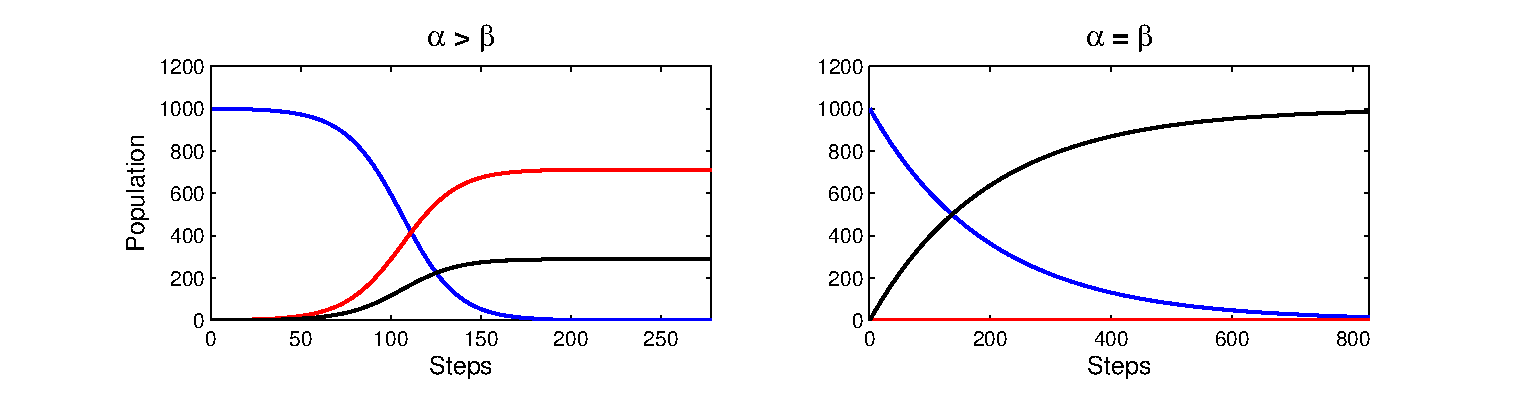
\includegraphics[scale=0.65]{../images/Matlab_figures/model-AgeB.eps}}
\caption{Doomsday scenarios for isolated states. Left: outbreak of zombies due to an unfavorable $\alpha/\beta$ ratio. Right: extinction of the human race with no zombie outbreak. In that limiting case, humans turn into zombies as fast as zombies get killed, but zombie-related deaths alone is sufficient to lead to annihilation of humans (\textcolor{blue}{blue} = susceptibles, \textcolor{red}{red} = zombies, black = removed. Left: $\alpha=1.6\cdot10^{-4}, \beta=1.0\cdot10^{-4}, \gamma=8.0\cdot10^{-5}$. Right: $\alpha=5.0\cdot10^{-3}, \beta=5.0\cdot10^{-3}, \gamma=8.0\cdot10^{-5} $). \label{deathS} }
\end{figure}

It is worthwhile noting that the doomsday scenario observed in both cases occurs irrespectively of the value of $\gamma$. The only effect of $\gamma$ is on the speed with which the human race gets wiped out from the surface of the earth. This makes sense since in both cases ($\alpha\leq\beta$) apparition of zombies occur at a rate greater or equal than they get killed and therefore they will eventually overcome our planet. The parameter $\gamma$ (which represent zombie-related death but not zombification) is only an additional way humans die but does not affect the zombie population. Another interesting observation one can make from figure \ref{deathS} is the different regimes when $\alpha<\beta$ and $\alpha=\beta$. In the first case we see a classical doomsday scenario where the zombie outbreak gradually leads to the disappearance of all humans with a few ``collateral'' damages as well. The second present an interesting feature. Indeed, no real zombie outbreak occurs (since we start with one zombie and the rate of zombification is equal to the rate of extermination) but the human population still disappears, triggered by the zombie-related death. This could be rationalized in the case where a small zombie niche would exist and humans would try over and over again to kill them but with each attack wave the number of infected would be equal to the number killed and other humans would be killed in the process as well. Finally, it is worth seeing that these two regimes would be the similar if a greater initial number of zombies were present, with the only difference that the convergence would be faster. 

Those two regimes represent the death of humanity. What would the parameters need to be in order to see the survival of the human race and what would it represent? From the relationship between the SZR parameters previously described, it is obvious that  for humans to survive in any case, the combined rates of their disappearance needs to be smaller than that of the killing of zombies ($\alpha+\gamma<\beta$). In the case where $\alpha<\beta$ (zombification slower than killing zombies) but  $\alpha+\gamma>\beta$ (overall humans still die at a greater rate due to the zombie-related death), the initial number of zombie matters in terms of outcome and survival of humanity. Those two regimes are shown in figure \ref{gamma_population}.



% Dependance to gamma and population
\begin{figure}[h!]
\centerline{
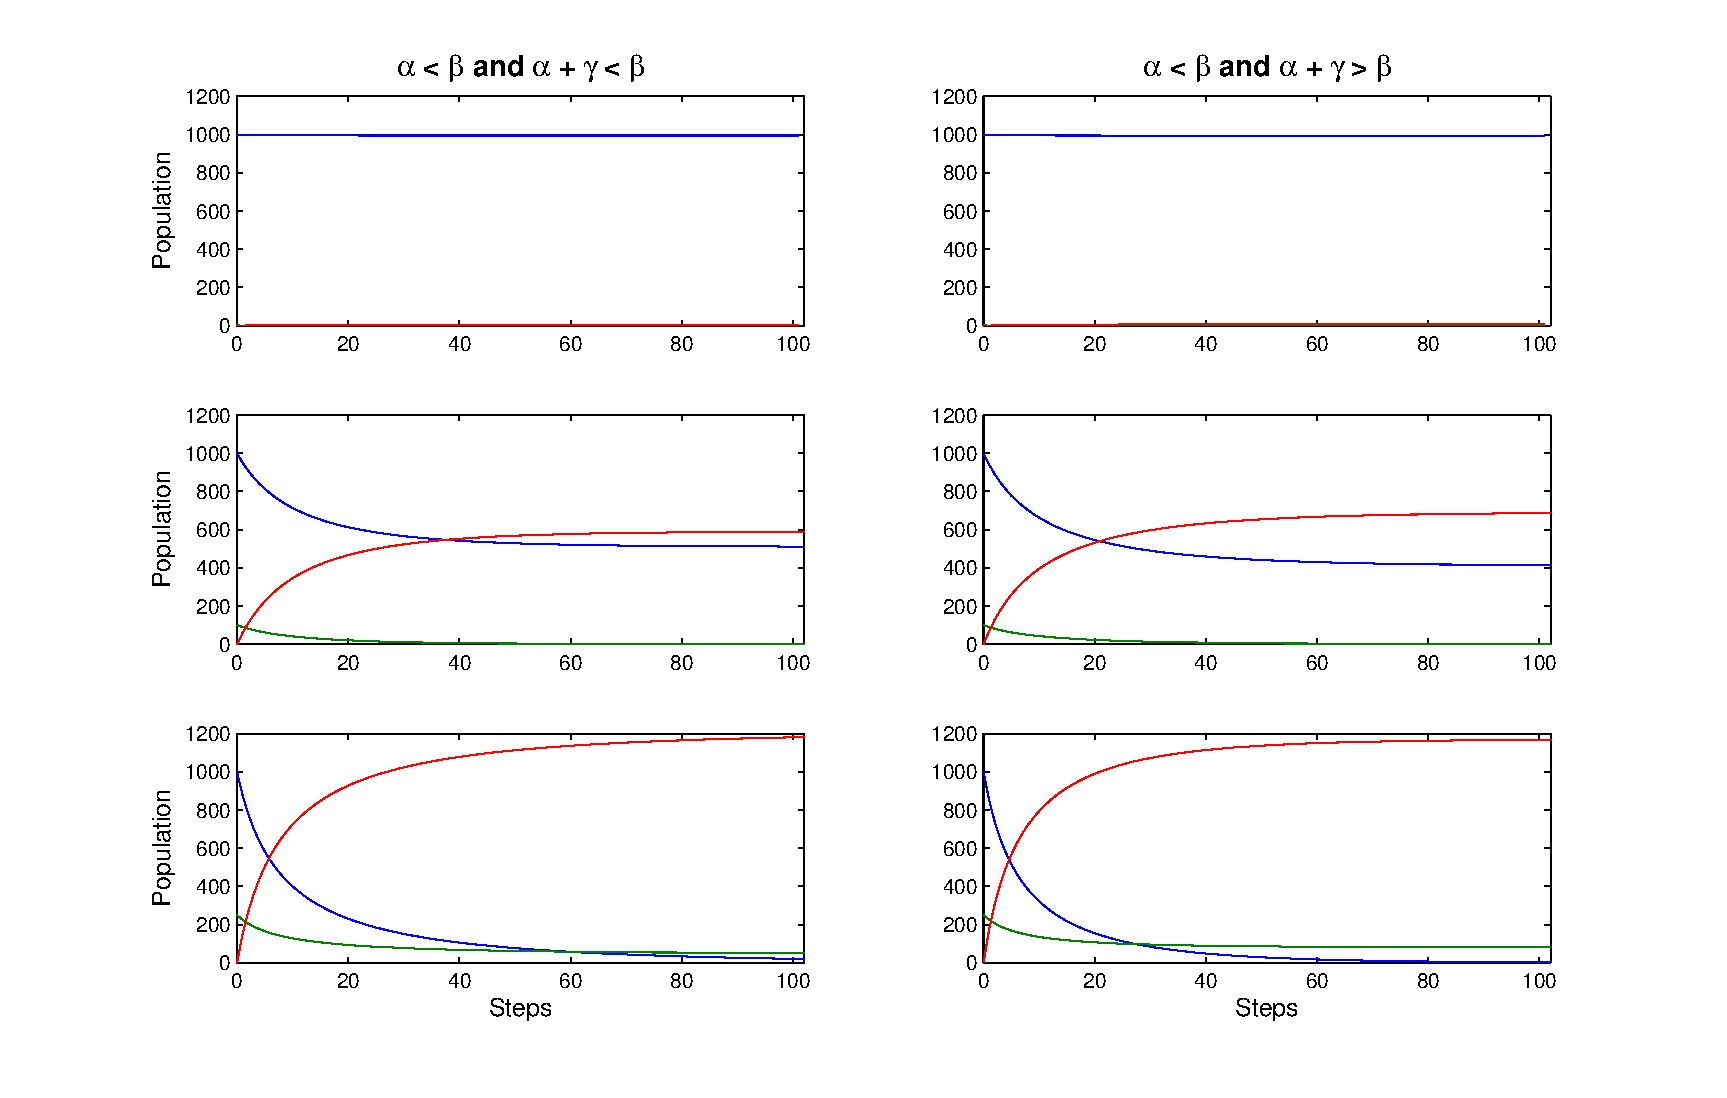
\includegraphics[scale=0.55]{../images/Matlab_figures/model-AltB.eps}}
\caption{ablaala(\textcolor{blue}{blue} = susceptibles, \textcolor{red}{red} = zombies, black = removed. $\alpha=4.0\cdot10^{-4}, \beta=5.0\cdot10^{-4}$ for all simulations. Left column: $\gamma=0.1\cdot10^{-4}$, right column: $\gamma=1.9\cdot10^{-4}$. Initial number of zombies: first line=1, second line=100, third line=200). \label{gamma_population} }
\end{figure}

It is visible that with a starting number of one or a hundred zombies, humanity survives in both cases. However, we can see that when the starting number of zombies is two hundreds, then the scenarios diverge and the situation where the overall death of humans is greater than the death of zombies (right column), then humanity disappears because the combined ``collateral''  deaths and zombification leads to a sharper decrease of the population of susceptibles, preventing the timely eradication of zombies. Furthermore, it is worth considering that the greater the initial number of zombies, even in the cases where humanity did not get anhiliated, the darker the outcome. Indeed, even if humanity survives, the outcome is not brilliant and most of our fellow human beings would have died. So for the brightest outcome possible, it is obvious that the the ratio $\alpha/\beta$ should be minimized.


\subsection{Population Time-Evolution with Connected States}\indent
\label{sec:time-evolv}
 
So far we have treated the SZR model in a closed system with no population exchanges with other states. We will now investigate the influence of population exchange at the macrostate level and see the influence on the outcome with respect to the choice of the inter-state fluxes ($\nu$ and $\eta$). 

Figure \ref{doomsday} represent a regime for our model where emergence of a single zombie in state 1 will ultimately lead to the total collapse of the world population by either zombification or death. This is an example of doomsday behavior at the international level. The left column represent population time-evolution for the different types of population (S, Z, R) in each state as well as for the world population. The right column represent the population variations at each step of the simulation. 
% Doomsday figure
\begin{figure}[h!]
\centerline{
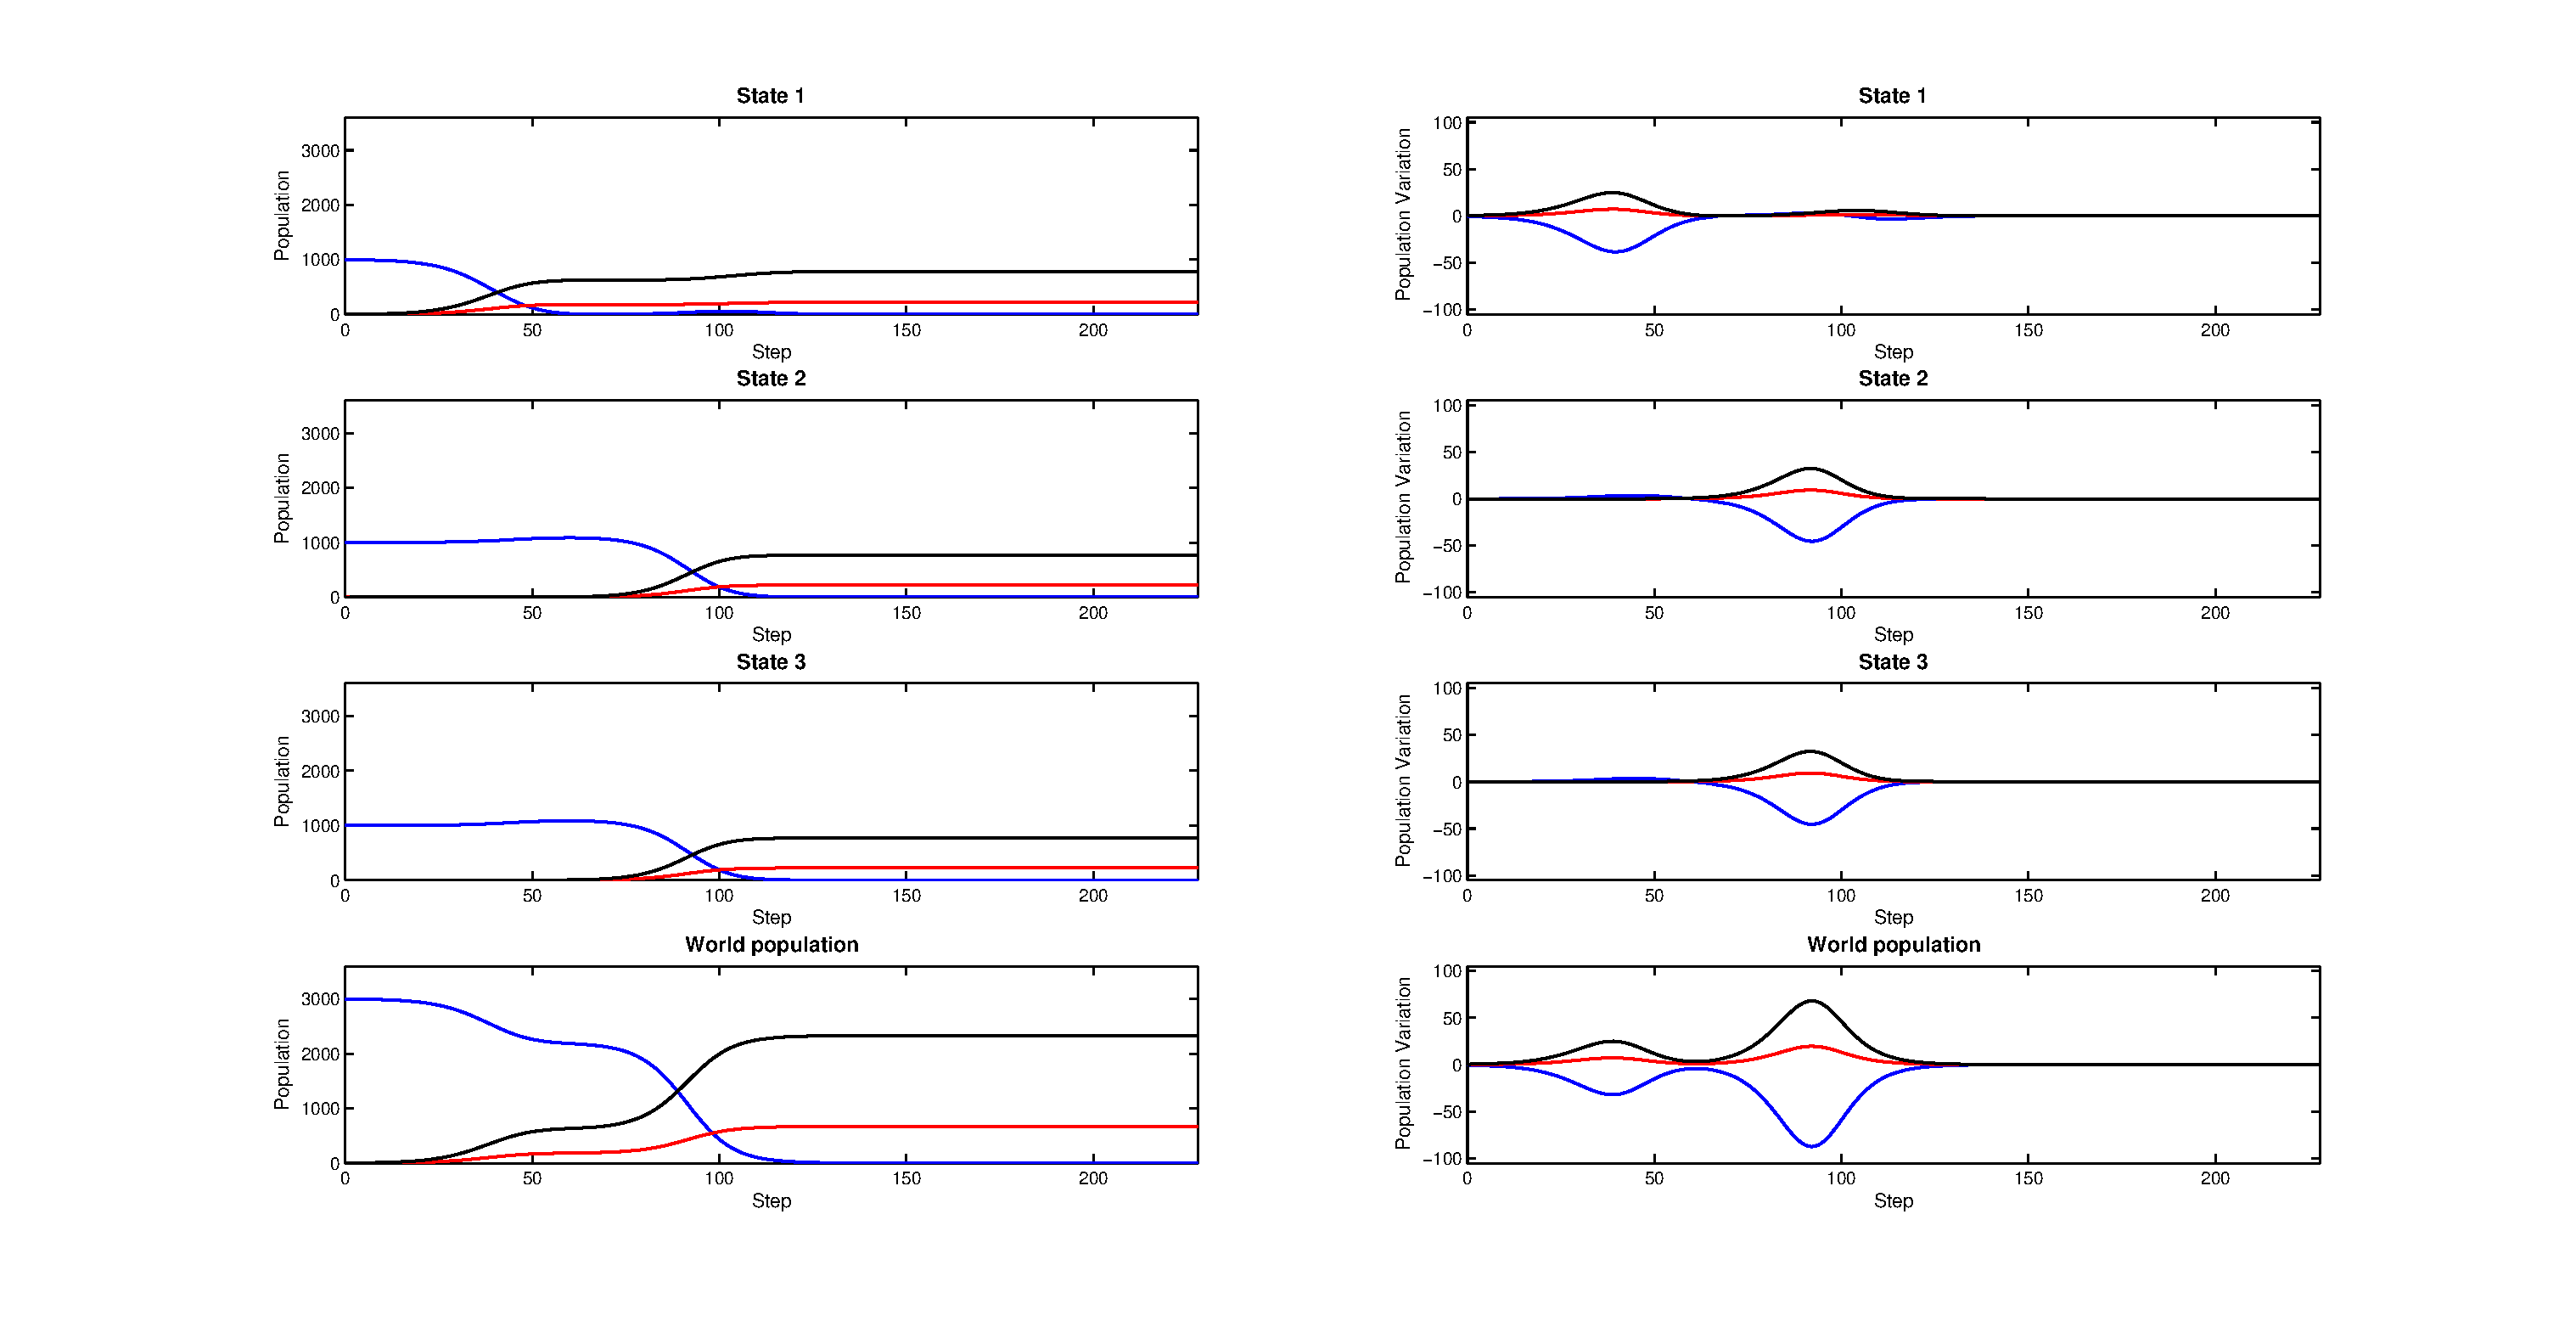
\includegraphics[scale=0.35]{../images/Matlab_figures/example_doomsday.eps}}
\caption{Doomsday scenario. Apparition of a single zombie in state 1 leads to full contamination of the world's population. Left panel represent the populations of each state (and world population) with respect to step number. Right panel represents the corresponding population variation (\textcolor{blue}{blue} = susceptibles, \textcolor{red}{red} = zombies, black = removed, $\alpha=1.5\cdot10^{-4}, \beta=5\cdot10^{-6}, \gamma=5\cdot10^{-4}, \nu=0.1, \eta=1.5\cdot10^{-4}$). \label{doomsday} }
\end{figure}

Interesting observation can already be made by looking at our model under such a regime. In particular, the delayed outbreak of zombies in state 2 and 3 due to the necessary build up of zombies and death of susceptible in state 1 to generate a ratio sufficient to be an incentive for the zombies to migrate to another state with more flesh. This is a direct consequence of our pseudo-flesh-craving model of the zombie in its migrational behavior. Although very weak, we can also observe a small emigration of susceptibles from state 1 to states 2 and 3. Moreover, one can observe that this flux is delayed with respect to the death of susceptible in state 1. Again, the explication of this macrostate-level behavior lies in our description of human migration based on a response to death in their state. In addition, the delay originates from the utilization of a sliding window, which is supposed to represent the lagging-time for people to react and the moment of inertia of large crowd migrations. Overall, we see that even with a parameter for susceptible migration ($\nu$) larger than the parameter for zombie migration ($\eta$) by three order of magnitude, the escape of susceptible from one state to the other is not sufficient for a survival of the human race. The explanation of it is likely two-fold: i) our description of human migration does not capture properly the expected behavior in the event of a zombie outbreak (massive exodus), ii) since $\alpha>\beta$, once a zombie crosses the border, the state is doomed to have its human population eradicated, no matter what (see \ref{szr}). 
% Zombie kill figure
\begin{figure}[h!]
\centerline{
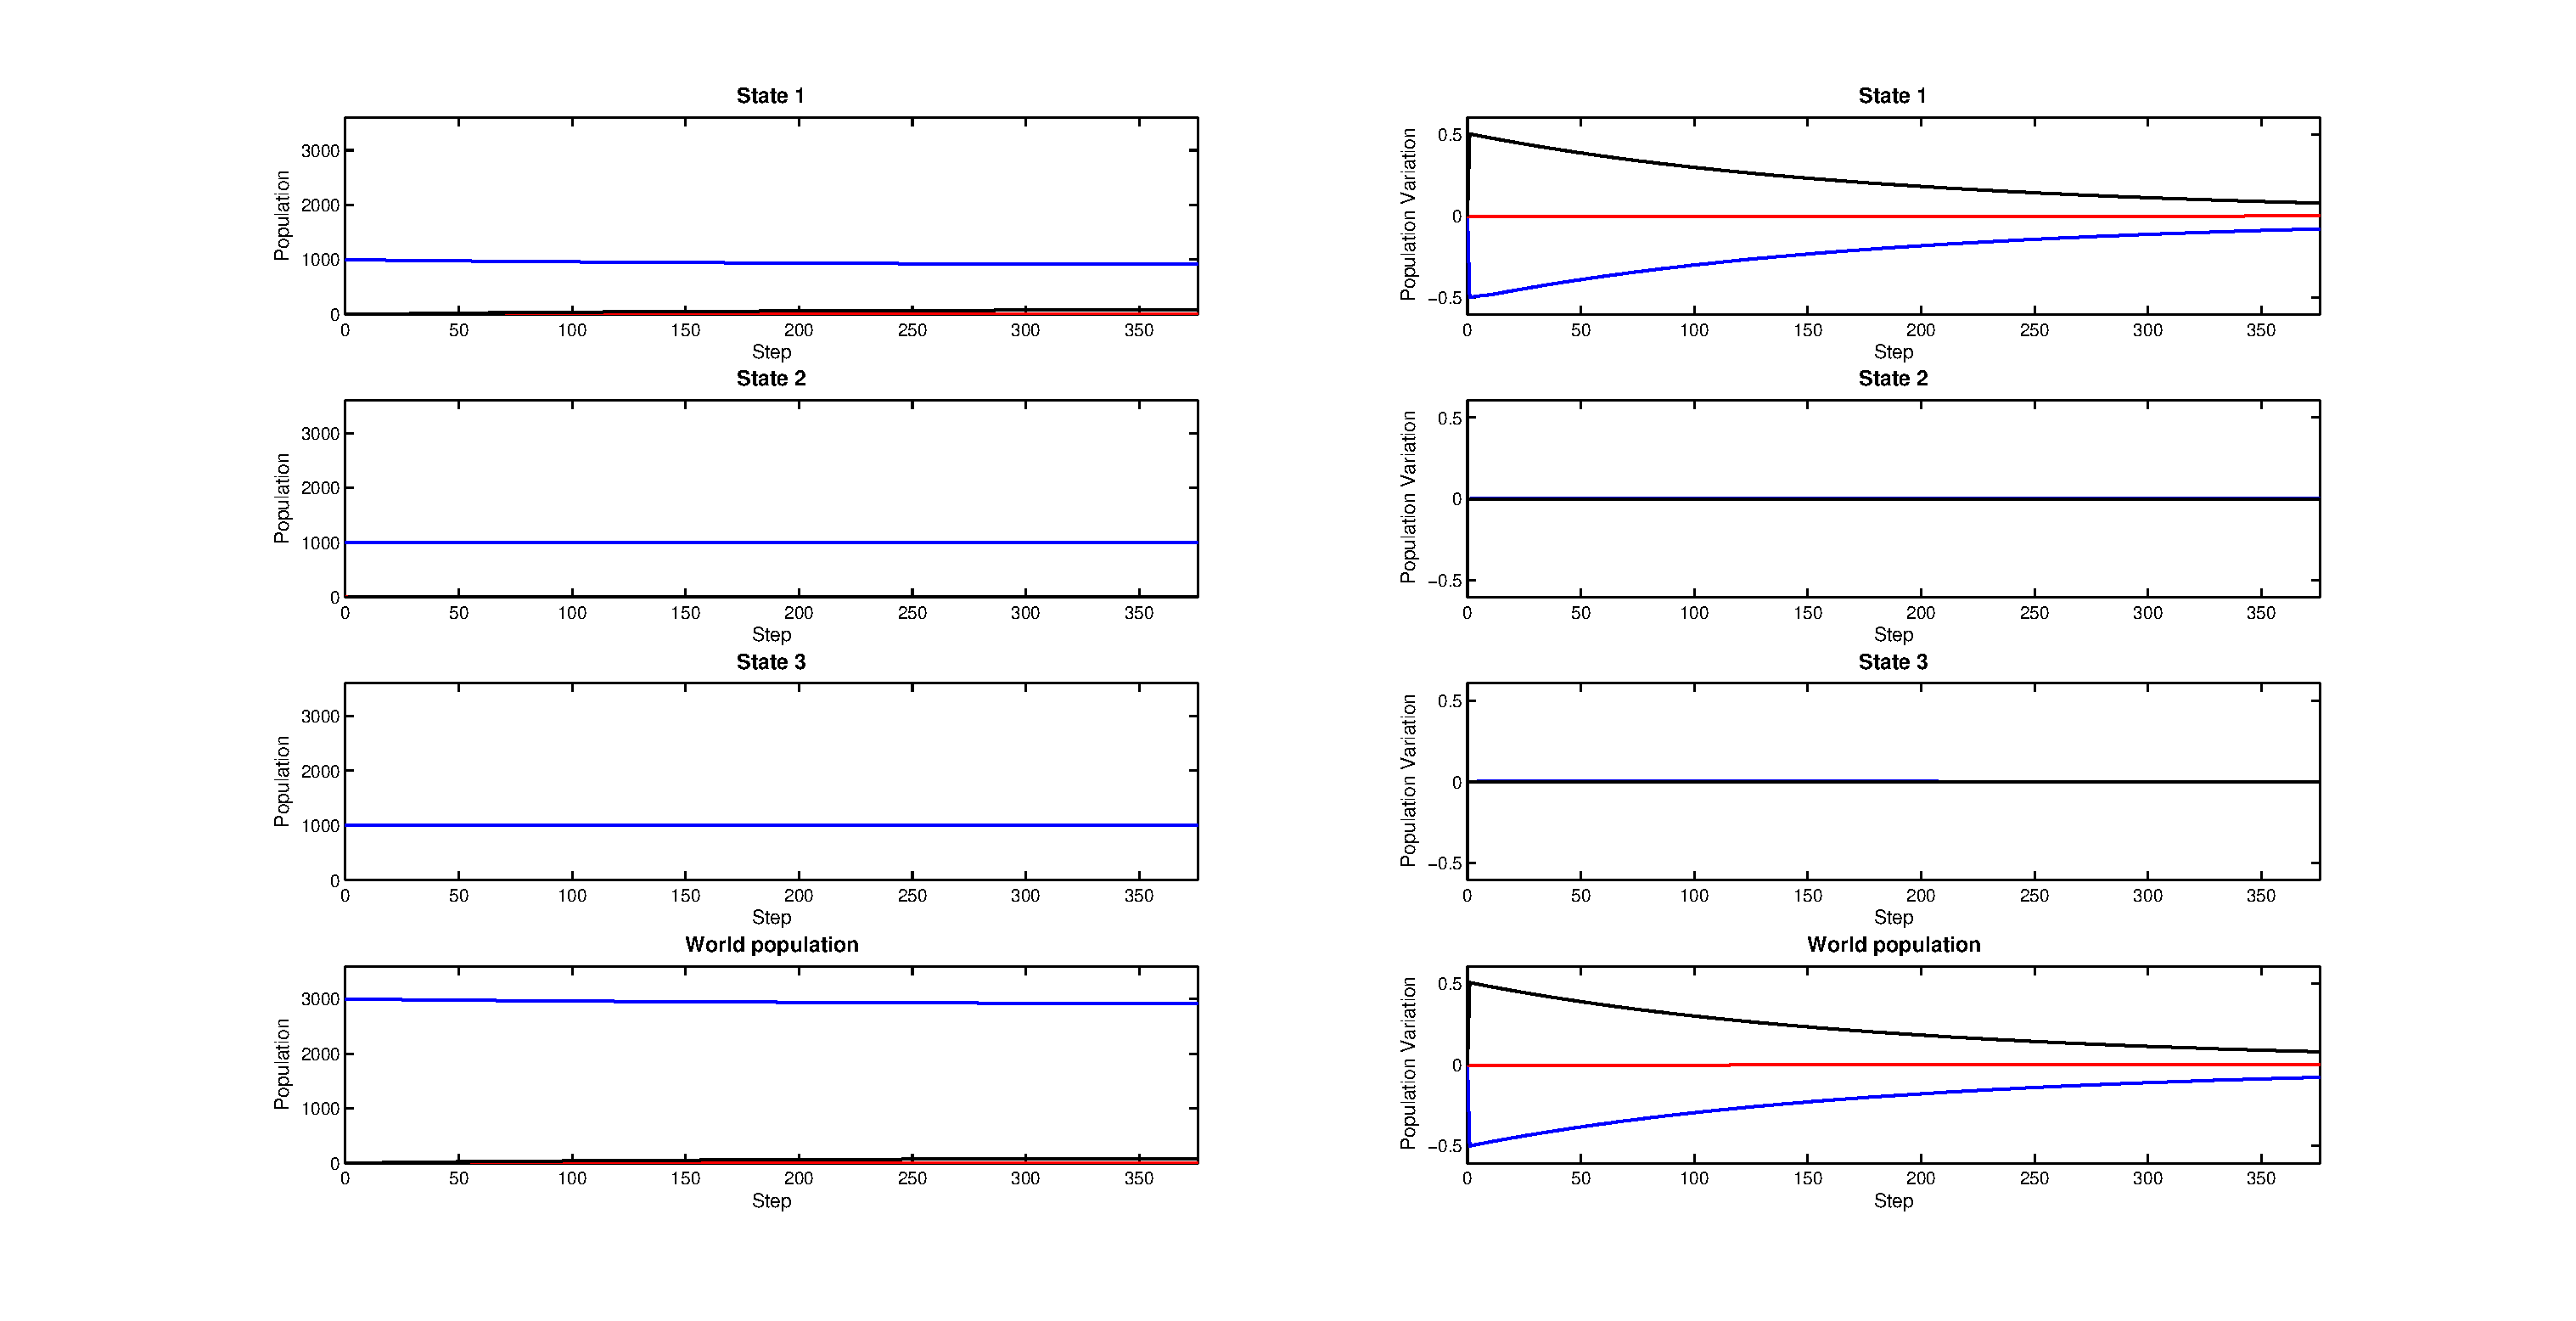
\includegraphics[scale=0.35]{../images/Matlab_figures/example_zkill.eps}}
\caption{Survival of humanity by zombie eradication. As soon as zombies appear in state 1, they get killed until the outbreak is contained. Left panel represent the populations of each state (and world population) with respect to step number. Right panel represents the corresponding population variation (\textcolor{blue}{blue} = susceptibles, \textcolor{red}{red} = zombies, black = removed, $\alpha=1.5\cdot10^{-8}, \beta=5\cdot10^{-6}, \gamma=5\cdot10^{-4}, \nu=0.01, \eta=1.5\cdot10^{-4}$).
\label{skill} }
\end{figure}

A regime where humanity would survive is shown in figure \ref{skill} where it can be seen that emergence of a single zombie in state 1 is not sufficient to generate an outburst due to the $\alpha/\beta$ ratio (see \ref{szr}). This situation is the international analog to what happened in figure \ref{gamma_population}. In such a scenario, the emergence of zombies in state 1 immediately gets eradicated, not allowing the build up of a zombie population that would trigger zombie migration. And even if it would, the fact that zombies get killed more rapidly than they appear, they would neither generate an outburst in the other states.




% Exode figure
\begin{figure}[h!]
\centerline{
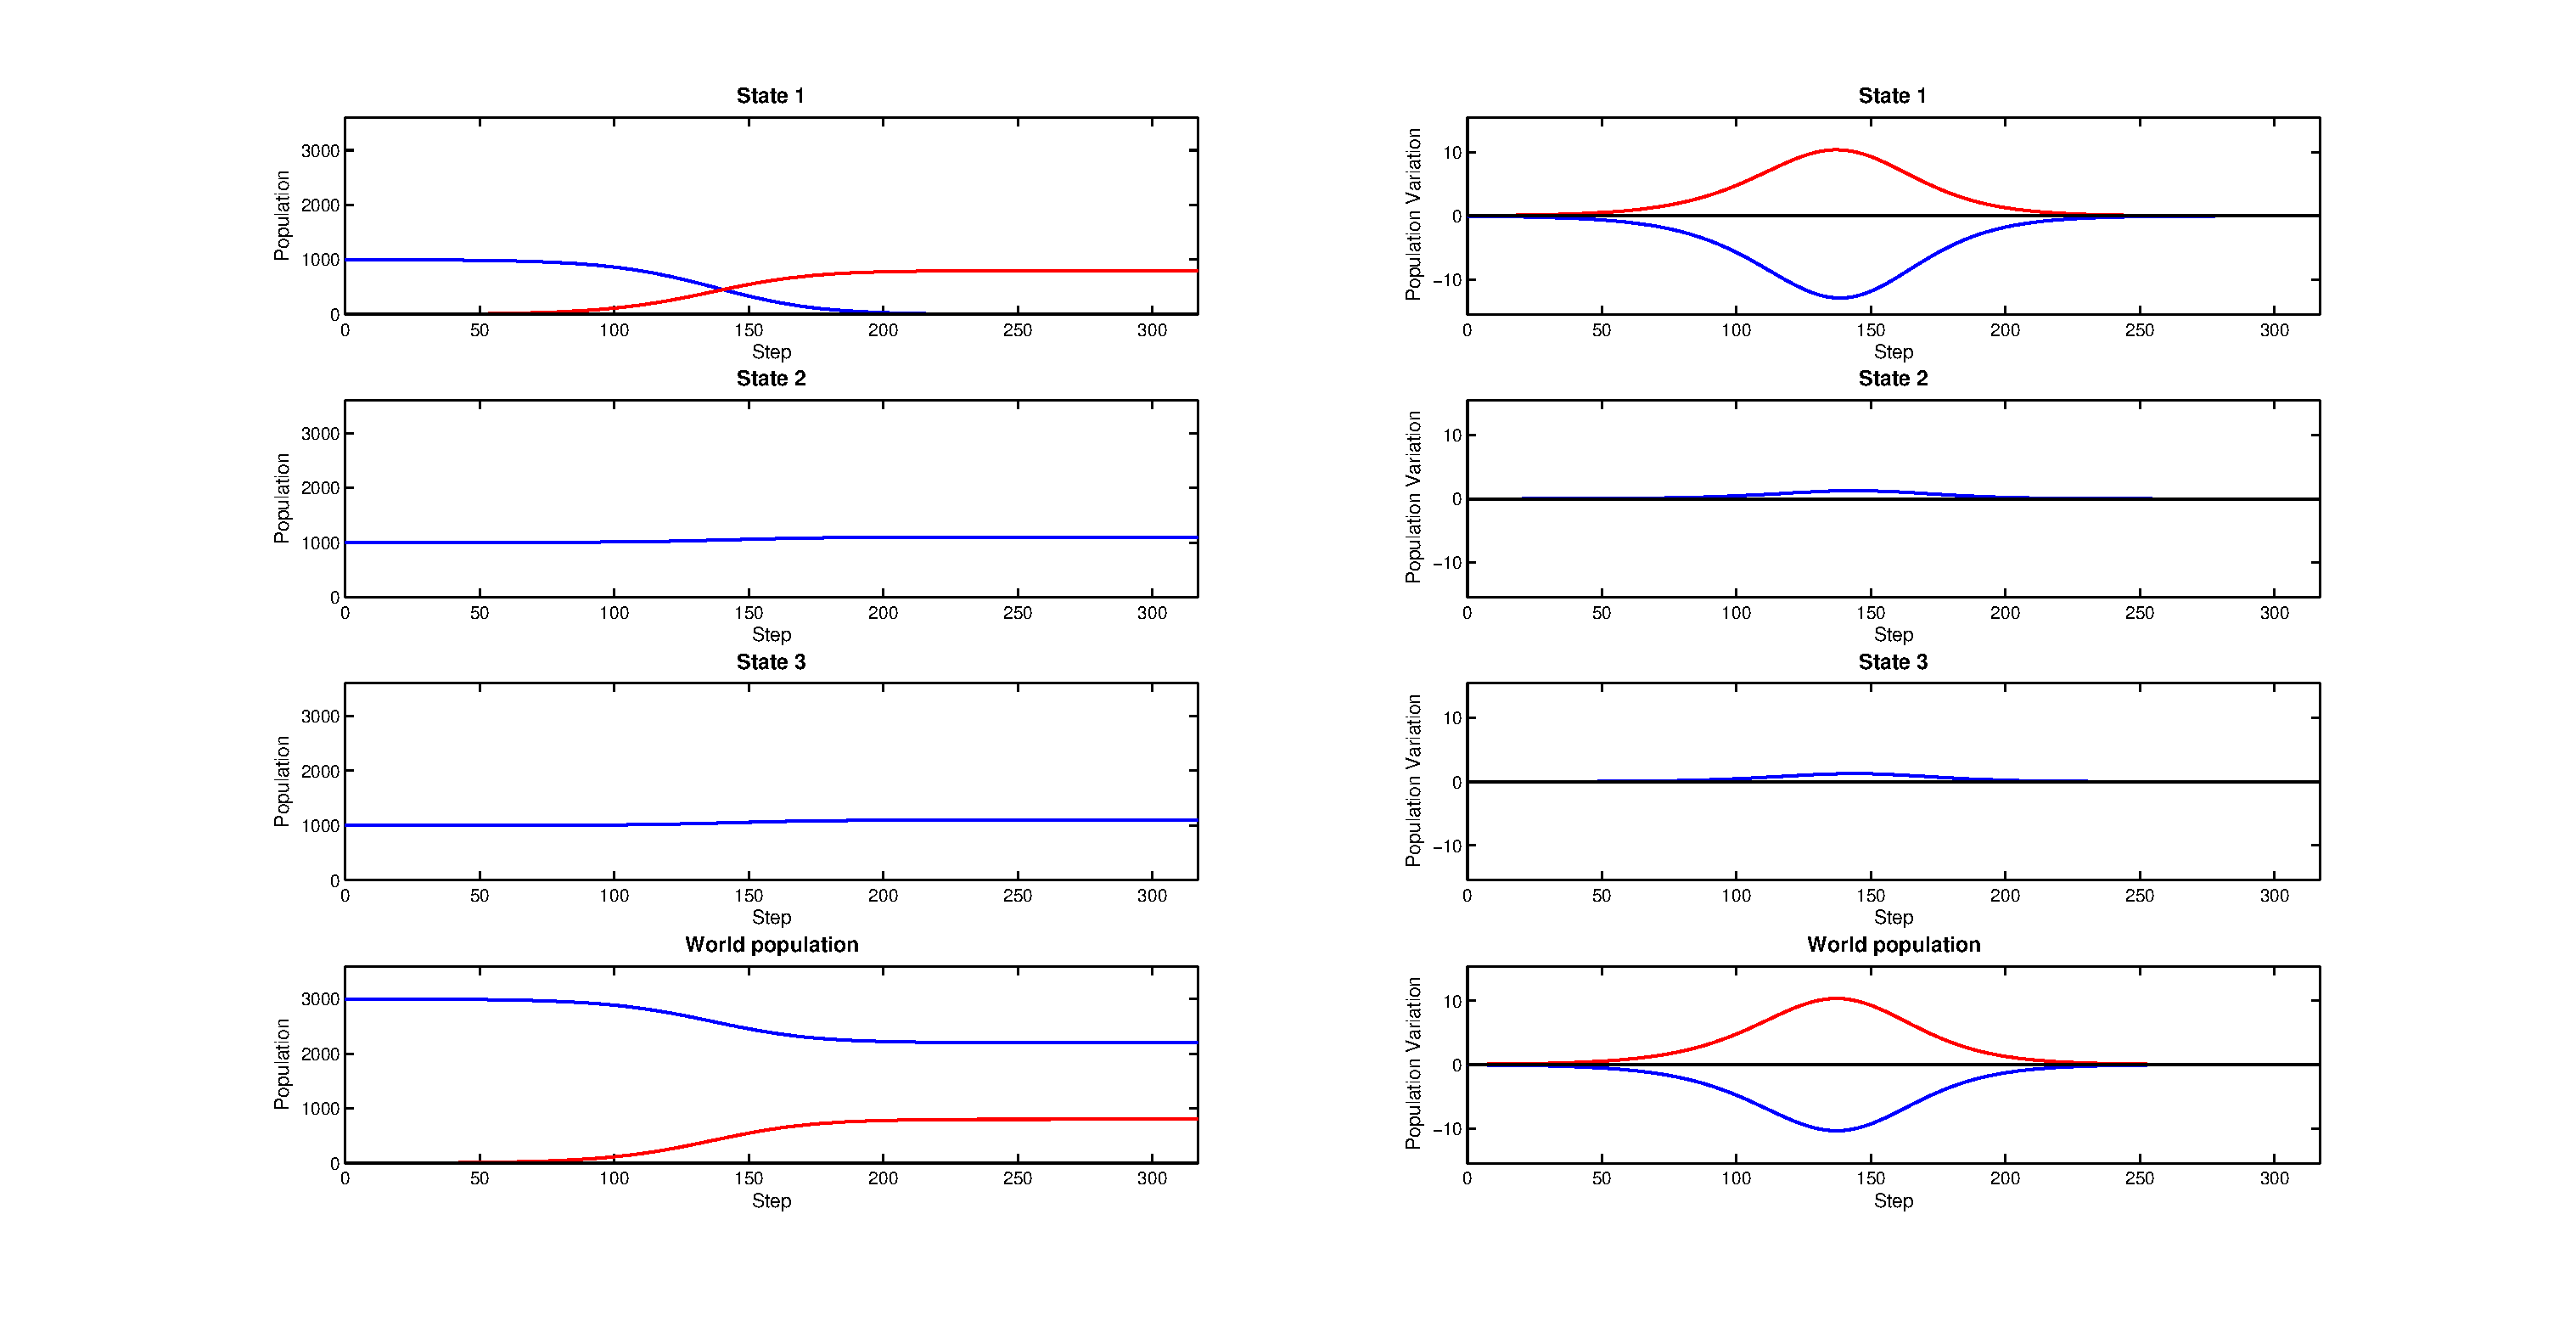
\includegraphics[scale=0.35]{../images/Matlab_figures/example_exode.eps}}
\caption{Survival of humanity and emergence of a zombie state. Emergence of zombies in state 1 leads to the exodus of the remaining population to states 2 and 3. State 1 becomes fully infested of zombies and the remaining of the world's population is in state 2 and 3. Left panel represent the populations of each state (and world population) with respect to step number. Right panel represents the corresponding population variation (\textcolor{blue}{blue} = susceptibles, \textcolor{red}{red} = zombies, black = removed, $\alpha=5\cdot10^{-5},  \beta=5\cdot10^{-10},  \gamma=5\cdot10^{-10},  \nu=0.1,  \eta=0$). \label{exodus} }
\end{figure}

Another example where humanity survives but for different reason is depicted in figure \ref{exodus}.
Here the set of parameters under scrutiny leads to an interesting phenomenon. Since $\eta=0$ and $\nu$ is large, emergence of a single zombie in state 1 triggers the outbreak and the build up of a zombie population. Consequently, humans start to feel the urge to move to another place, which they do but since the borders are closed to zombies ($\eta=0$) they can not infest another state. As a result, all remaining susceptibles from state 1 migrate to the other states and the initial place of the outbreak becomes a zombie-only state. Such a case can be viewed as a special case of quarantine where an entire country would become depleted from its human inhabitants to the profit of a new population; zombies. Interestingly, this scenario had been postulated by Drezner for a zombie outbreak in a liberal world \cite{drezner}. 

\subsection{Phase Transition for the Micro- and Macro-State Parameters }\indent

So far we have treated specific set of parameters, which displayed interesting regimes with different outcomes for our model. The next question is to understand the full dependance of every parameter with respect to the others in order observe the phase transition of location of the interesting regimes of our model. As mentioned before, a complete parameter sweep would not be feasible due to the high number of connected parameter present in our system (all of them). Accordingly, we rationalized that since we deconvoluted the behavioral treatment of the micro and macro state we could do the same with the parameter sweep. We first swept $\alpha$, $\beta$ and $\gamma$ under three conditions of $\eta$ and $\nu$ to see the phase transition at the microstate level and then took a point in this phase-space that presented interesting properties to do a parameter sweep of $\nu$ and $\eta$. The idea was to find sets of microstate parameters and then see how modifying the macrostate parameters would influence the outcome of simulation, \textit{i.e.} how modifying foreign policies could save humanity.
% 3D plots for alpha beta gamma
\begin{figure}[h!]
\centerline{
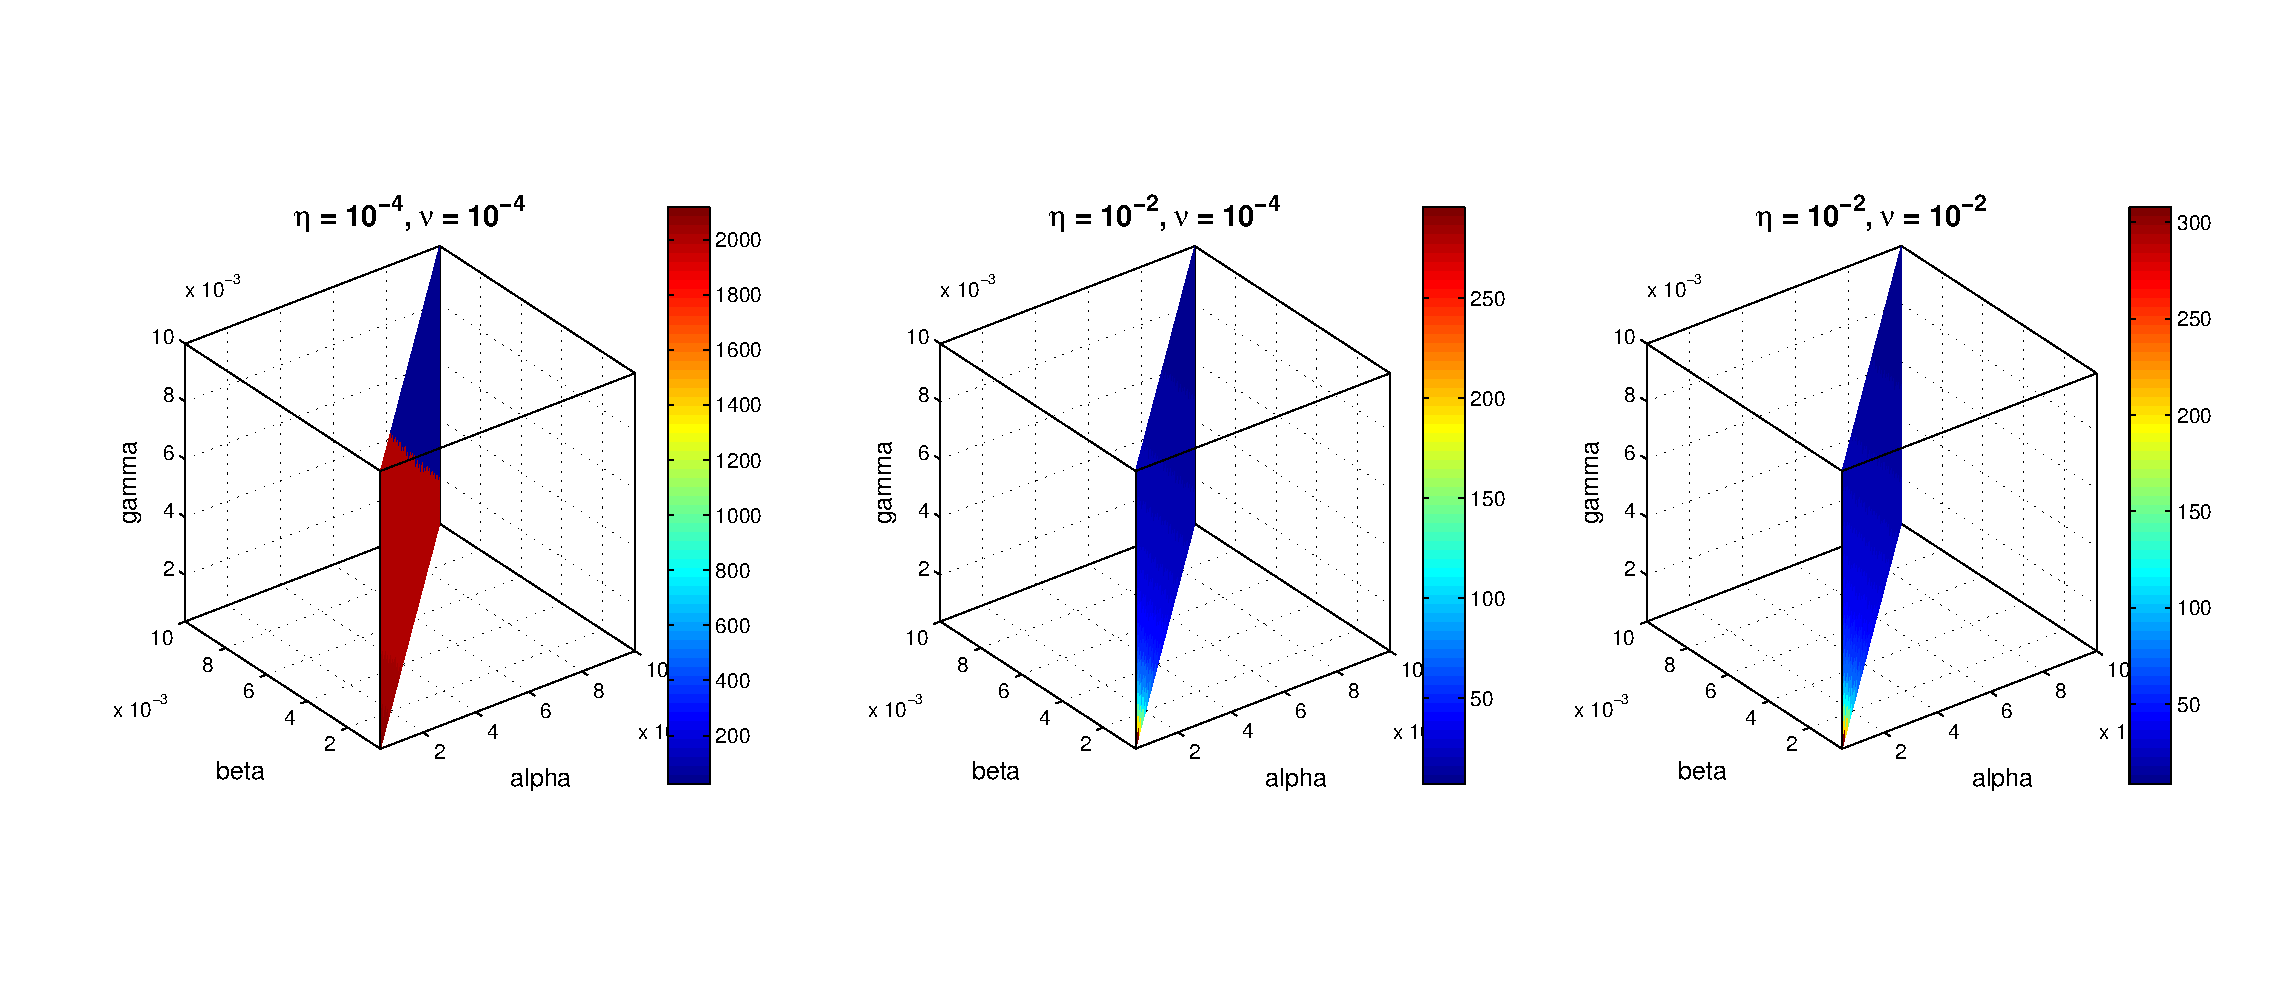
\includegraphics[scale=0.45]{../images/Matlab_figures/a-b-g-sweep.eps}}
\caption{Parameter sweep for $\alpha$, $\beta$ and $\gamma$ under different $\nu$ and $\eta$. Plotted surface represent the phase-transition between simulations with survivors and simulation with none. The color bar represent the number of humans who survived for each of those cases.  \label{a-b-g} }
\end{figure}

Figure \ref{a-b-g} shows the parameter sweep for $\alpha$, $\beta$ and $\gamma$ with different fixed $\eta$ and $\nu$. The surface plotted represent the simulations that had a non-zero human population at the end but a neighbor in the matrix for which it was the case (see \ref{sec:findTransition} for details). Hence, those surfaces represent the surface transition for sets of $[\alpha, \beta, \gamma]$ between regions of the phase-space where humanity did not survive and regions where it did. Interestingly, we can observe that in all three cases we see a linear relationship between the effect of $\alpha$ and $\beta$ (median plan through the 3D matrix), while the effect of $\gamma$ is negligible. The sharp color transition on the plan for the left graph of figure \ref{a-b-g} is likely due to an artifact of our implementation and not a physically meaningful result. Indeed, as safeguard we implemented a stop of the simulation in the case of S and Z mean population fluctuation becoming lower than a threshold (see \ref{outbreakimpl}). It is likely that changing a little bit the value of $\gamma$ in this region can switch between an artificially ended simulation due to low fluctuation to simulations that end by convergence. We then decided to chose a point on this transition-surface and use this $[\alpha, \beta, \gamma]$ triplet to sweep parameters $\nu$ and $\eta$ in order to see the transition phase of those parameters under a fixed $[\alpha, \beta, \gamma]$ triplet of interest (because itself located at a phase transition).
% Heat map of eta nu sweep
\begin{figure}[h!]
\centerline{
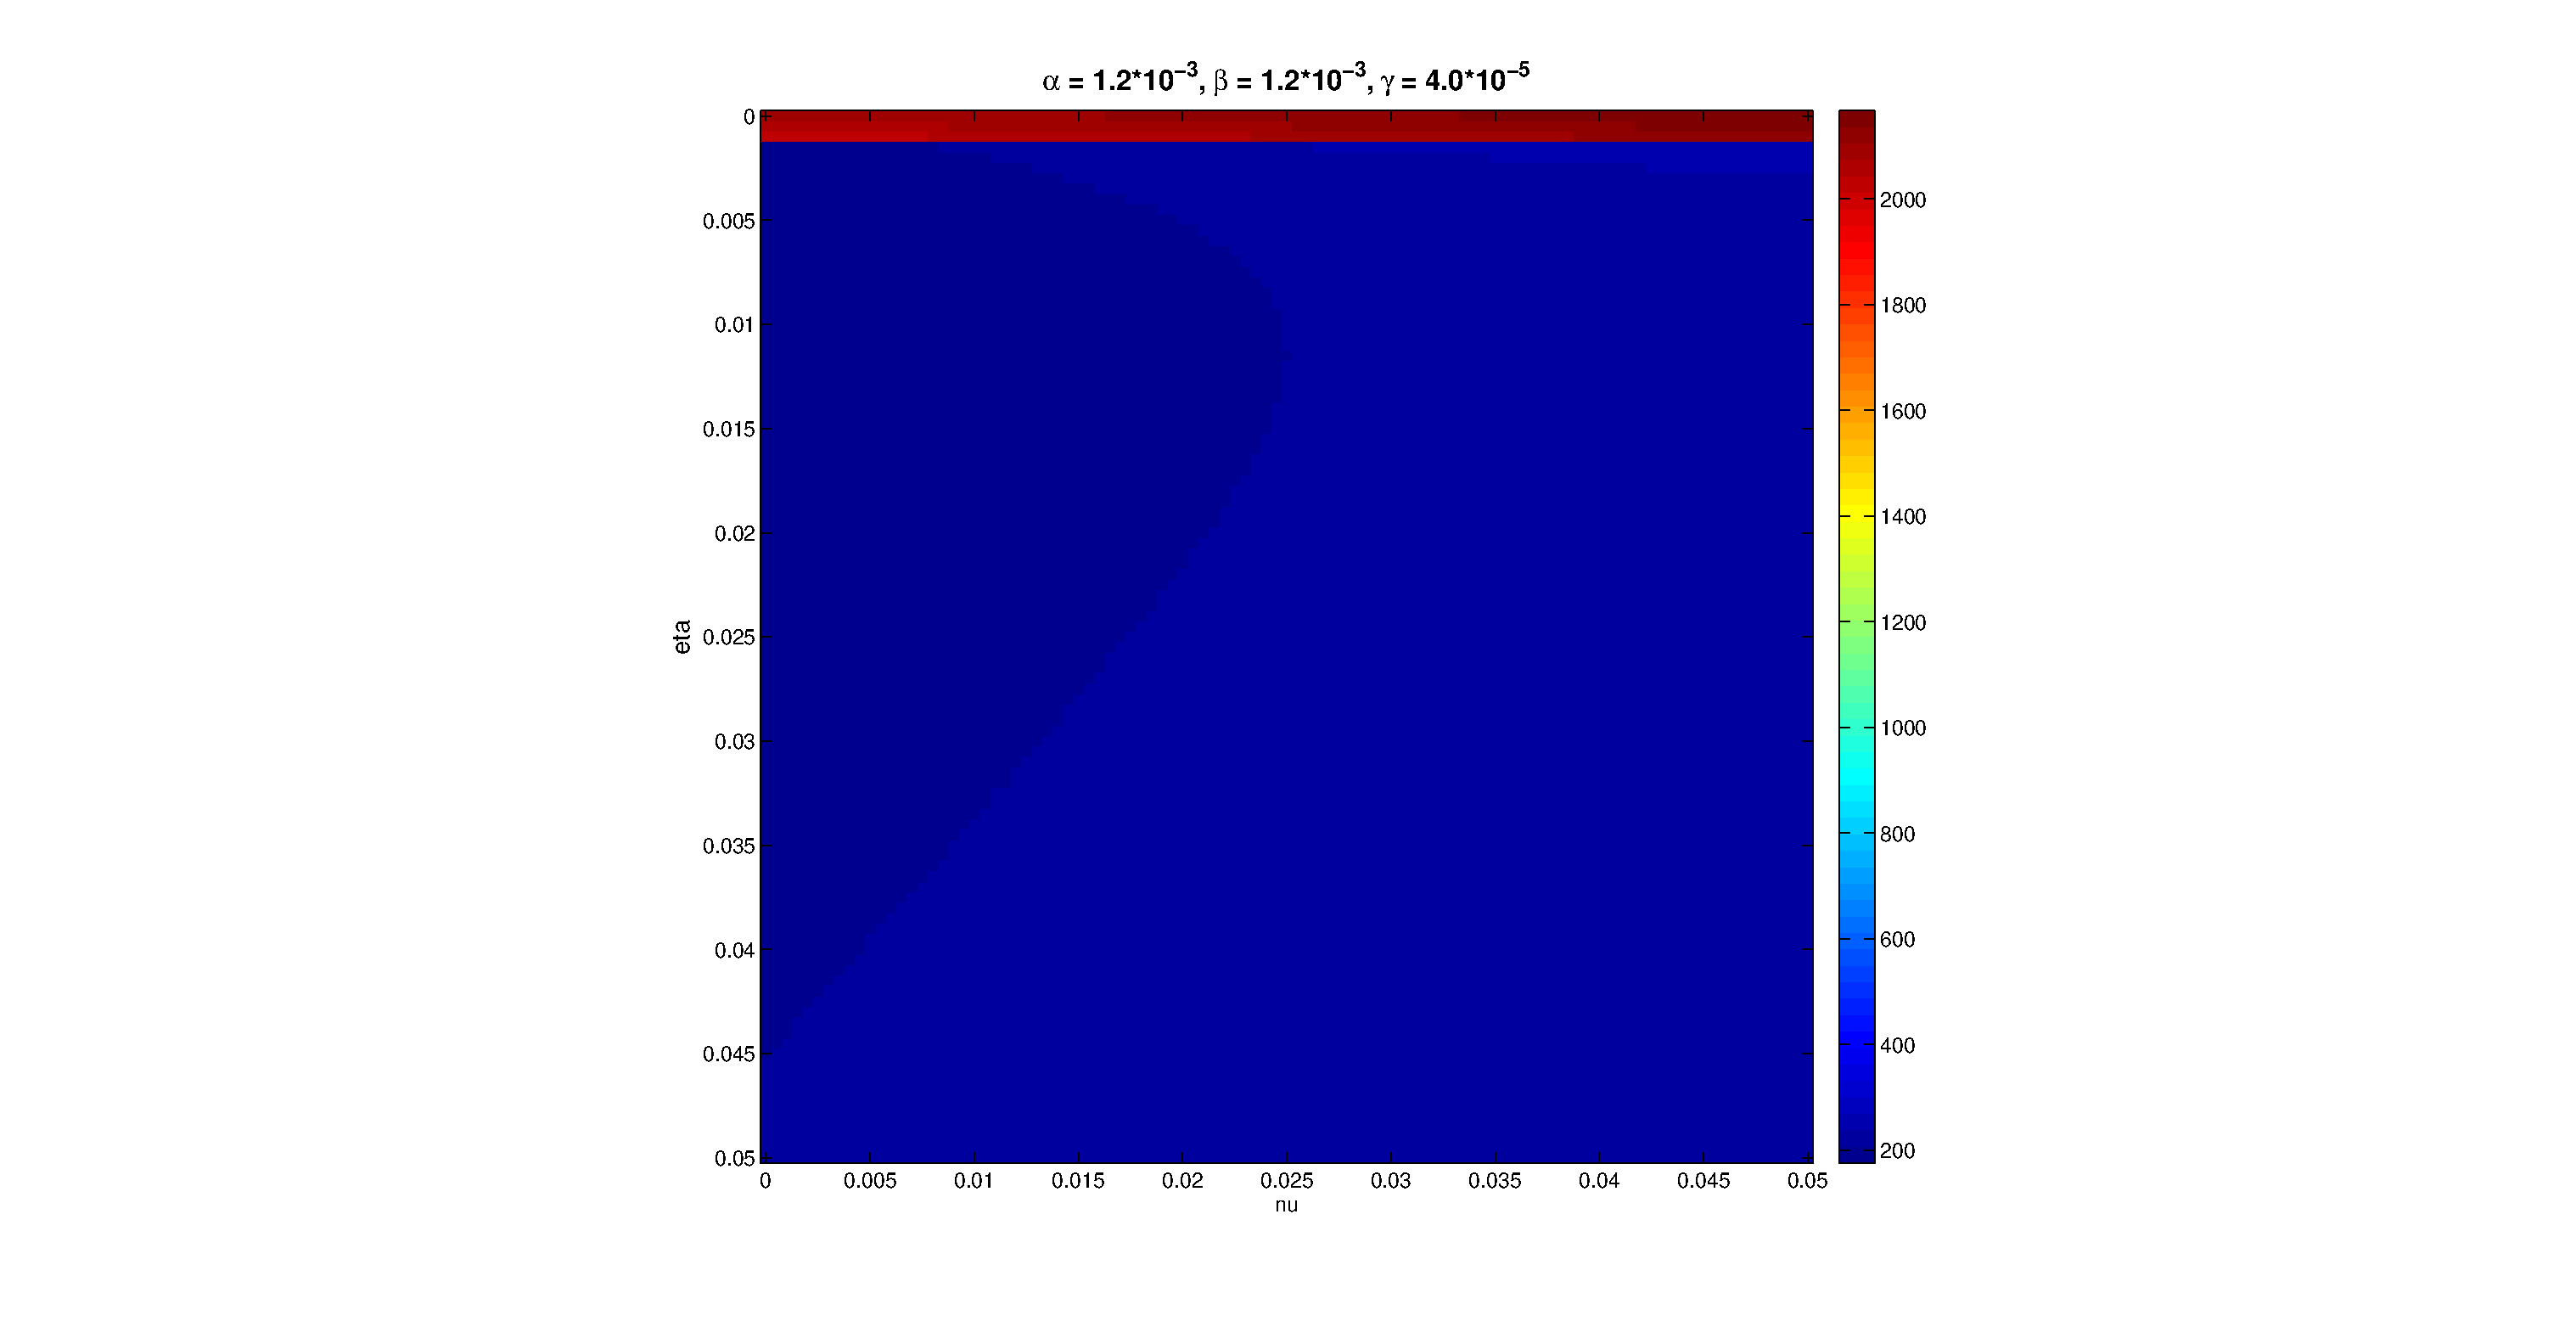
\includegraphics[scale=0.33]{../images/Matlab_figures/nu-eta-sweep.eps}}
\caption{Parameter sweep for $\nu$ and $\eta$ under a fixed  $[\alpha, \beta, \gamma]$ triplet. The color bar represent the number of humans who survived for each simulation.  \label{nueta} }
\end{figure}
Figure \ref{nueta} shows the heat-map for this parameter sweep. It is worth noting that the upper band of the heat-map that represent a high number of survivor is not really a phase transition but more a limit of our model with the parameters under consideration. Indeed, it represent the case were the transfer of zombie is zero or almost inexistent, making the contamination of the other state impossible (hence the high number of survivors). For the rest of the phase-diagram, we observe a biphasic system. The reason for this behavior is unclear, in particular the absence of a real gradient but it might be due to the threshold value used to stop the simulation when fluctuation became small. 



\subsection{Asymmetry in State Power}\indent

So far we have only looked at fully symmetrical systems where both populations and parameters under scrutiny were chosen equal for every state. We did so in order to avoid introduction of additional effects on the simulation outcomes, which would have been hard to deconvolute from the rest of the features of our model. Another reason was that certain parameters simply represent ``physical constants'' of zombification, \textit{i.e.} they are independent of the state under consideration and are only related to the zombie outbreak paradigm under consideration. Parameters that fall into this category are typically $\alpha$ and $\gamma$. Indeed, it is likely that zombification will occur at the same rate everywhere since it is an epidemiological parameter and therefore should not be influenced by factors such as socio-economical environments. Under the assumptions of our model, the same consideration hold for $\gamma$. Parameters $\nu$ and $\eta$ could arguably be different between states but for the sake of simplicity, we decided to model cooperation in systems of homogenous international relationships. Finally, $\beta$, which represent the efficiency of the people of a given state to kill zombies, was so far set as identical in all systems for symmetrical reasons. However, a more accurate representation of the international scene implies considering a world containing states possessing different military powers. A simple way to represent such an effect within the framework of our model would simply be to assign different $\beta$ to the three states. Figure \ref{basym} represents such a case, where state 3 possess a value for $\beta$ one order of magnitude higher than states 1 and 2. 
 
\begin{figure}[h!]
\centerline{
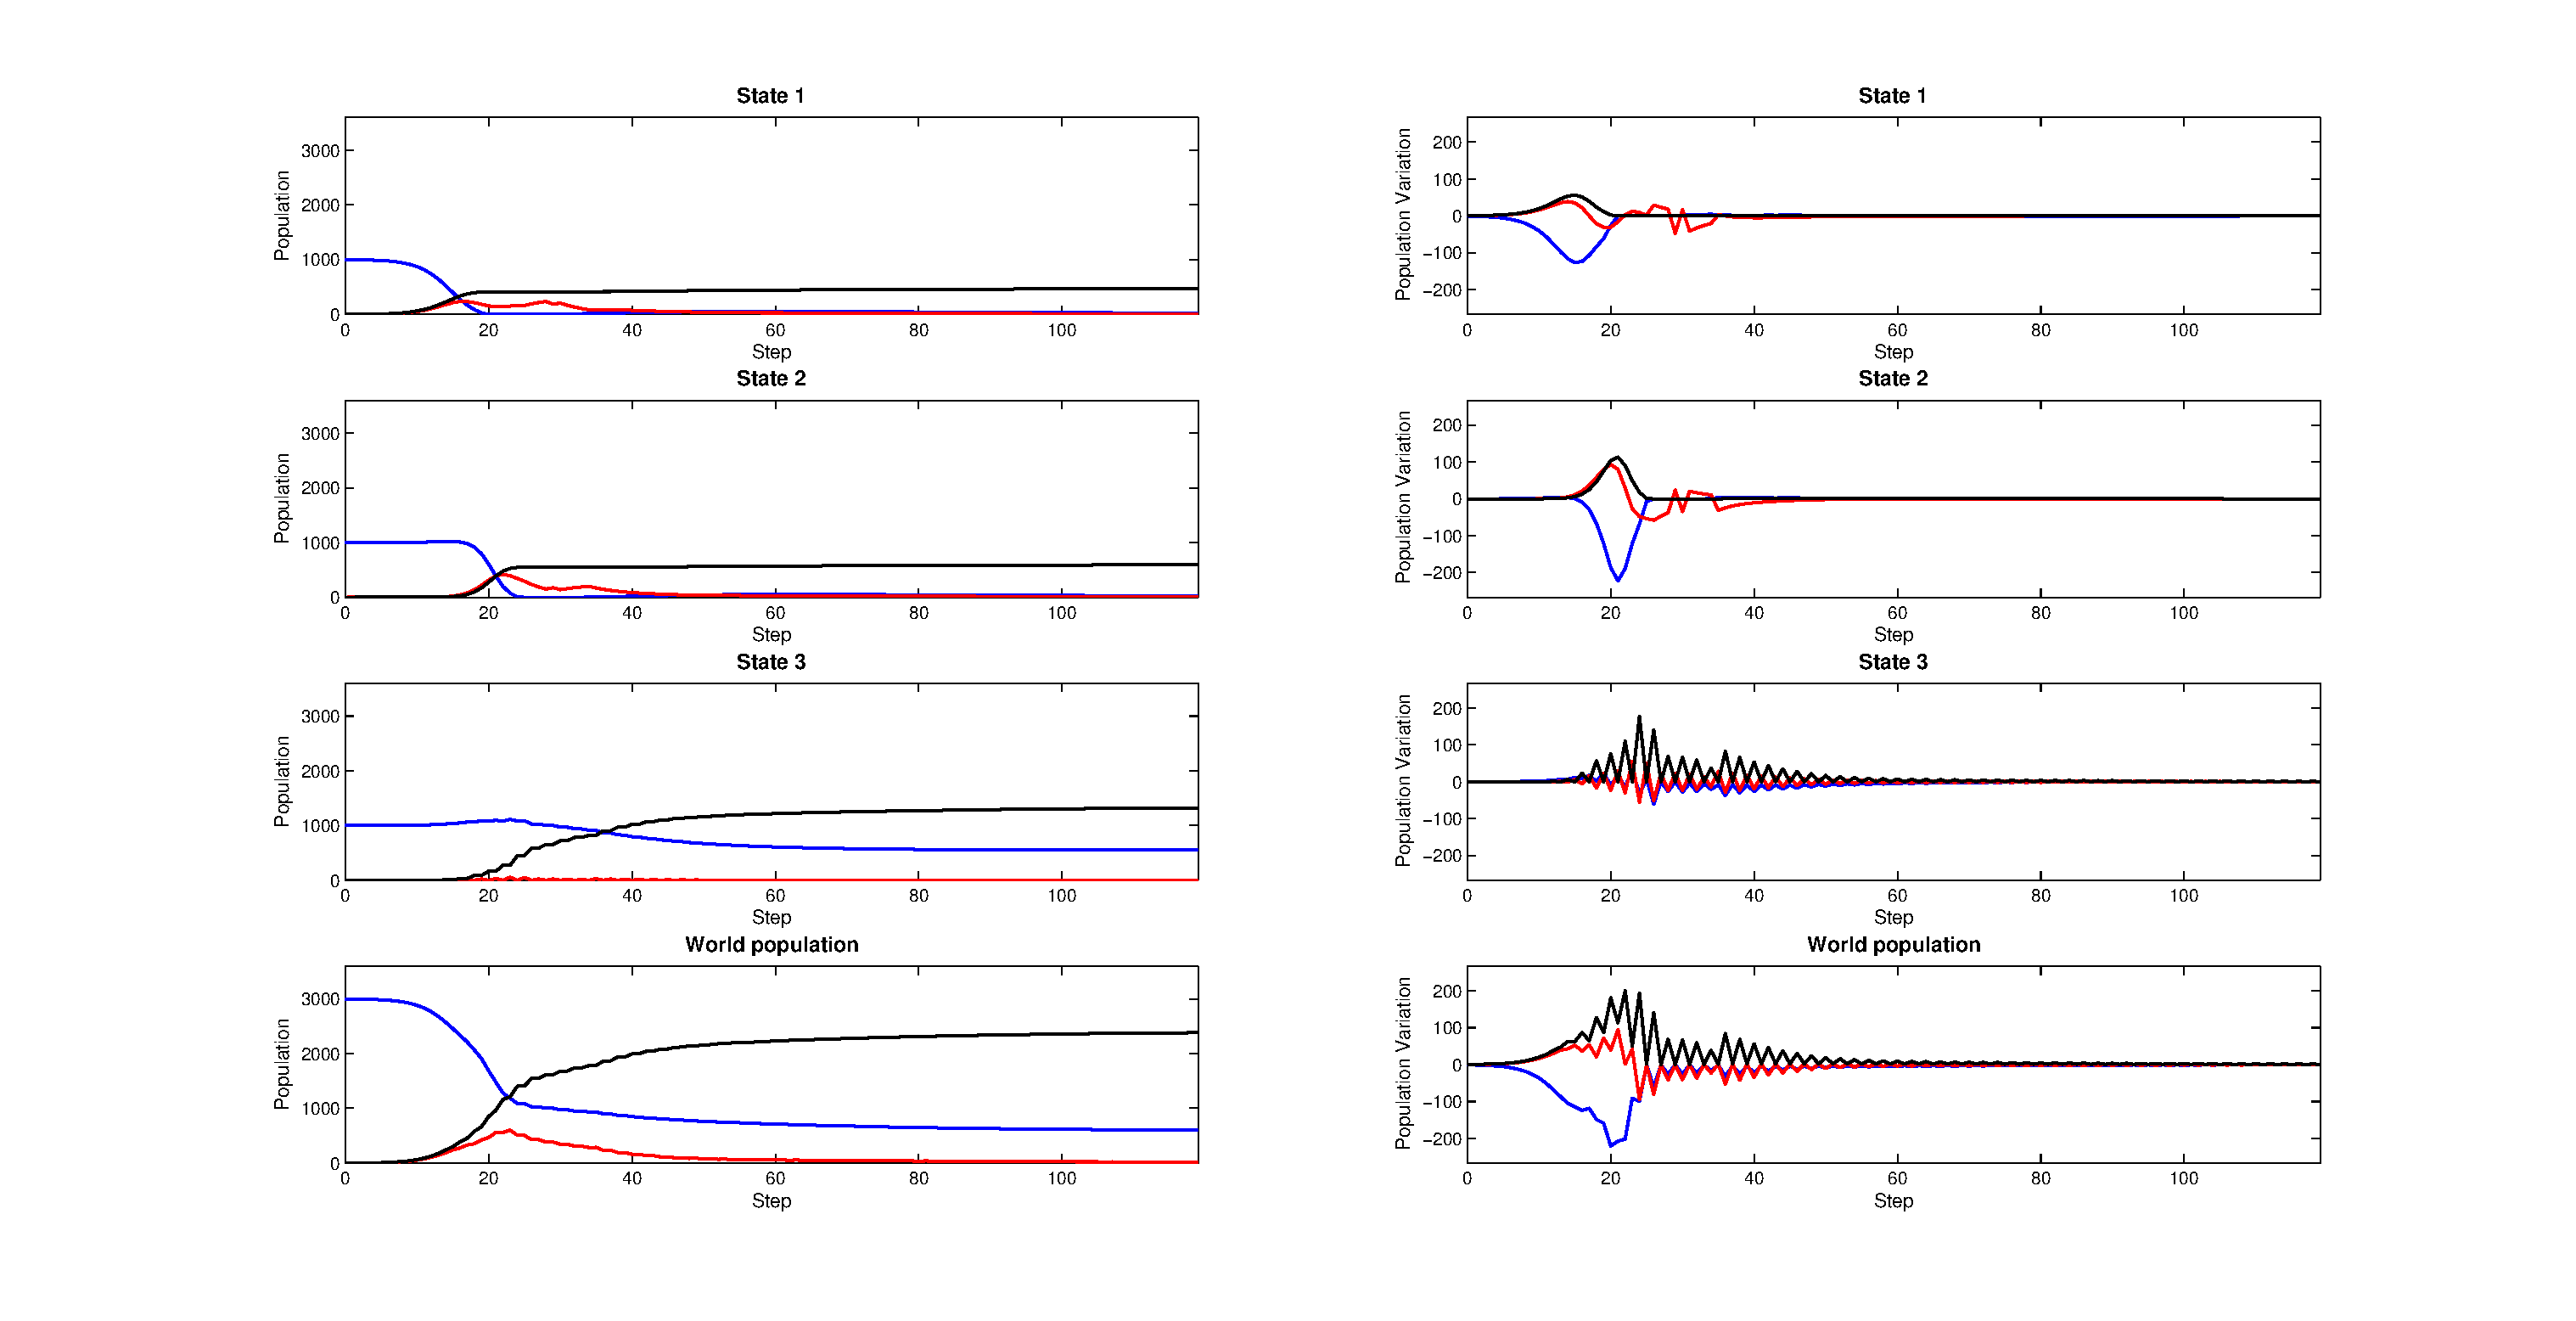
\includegraphics[scale=0.35]{../images/Matlab_figures/asymmetric-system.eps}}
\caption{The effect of asymmetry in state power.  Emergence of zombies in state 1 leads to contamination and partial death in states 1 and 2, leading to the emigration of both susceptibles and zombies to the other states.  State 3 possessing a higher $\beta$ value than the other states, the outbreak is crushed at the border, leading to zombie eradication. Left panel represent the populations of each state (and world population) with respect to step number. Right panel represents the corresponding population variation (\textcolor{blue}{blue} = susceptibles, \textcolor{red}{red} = zombies, black = removed, $\alpha=1.0\cdot10^{-3}, \beta=5\cdot10^{-4} $ (states 1 and 2) $\beta=5\cdot10^{-3}$ (state 3) $, \gamma=1\cdot10^{-4}, \nu=0.25, \eta=0.1$). \label{basym} }
\end{figure}

Such a system displays interesting features. First of all, it is worth noting that since $\alpha>\beta$ in state 1, a zombie outbreak occurs, leading to contamination and death of the susceptibles in this state. A similar effect is observable for state 2 for the same reason, however with a delay (accumulation of zombies in state 1 before they start emigrating). Those features are consistent with the observations made in section \ref{sec:time-evolv} and figure \ref{doomsday}. Indeed, $\alpha$ being greater than $\beta$, zombies appear with a rate higher than their eradication, leading to disappearance of humans in those states. Emigration of susceptible is also observable after the zombie outbreak. But most interestingly, it can be observed that the higher value of $\beta$ in state 3 (with $\beta>\alpha$ unlike state 1 and 2) allows to avoid a zombie outbreak in this state. Moreover, and contrary to the case observed in figure \ref{exodus}, apparition of a zombie state does not occur. Indeed, once state 1 and 2 are depleted from their susceptibles, zombies start emigrating to state 3 where they immediately get killed at the border, eventually leading to full eradication of all the zombies. This behavior provides an interesting modeling of a case where an outbreak would lead to people fleeing and finding refuge in another state where the fate of humanity would be decided in a total war against zombies until none remain.





% SUMMARY AND OUTLOOK
\newpage
\section{Summary and Outlook}\indent

In the present study we showed the behavior of a model of interconnected SZR model as a way to represent international cooperation. We investigated the role of the inter-state connections as described by our model for the survival of humanity in the event of a zombie outbreak. Due to the lack of empirical precedent or literature data available on the subject, it has been hard to define a model that could grasp the complexity of such a scenario on the international scene. In particular, we encountered problem in the modelisation of the macrostate level fluxes due to the high inter-connectivity of the equations, which led to implementation difficulties. The model described here represent the population evolution at the microstate level with a fairly standard epidemiological treatment while the macrostate level is described by a reaction-based migration of susceptible with inertia and a pseudo-flesh-craving paradigm for the transfer of zombies. Due to the lack of data that could have allowed us to generate the parameters needed for our description, we had to do a parameter sweep to find the phase transitions. Here again we encountered difficulties due to the high dimensionality of our system. We tackled this problem by treating the parameter sweep of the microstate and macrostate as almost independent. 

Although they did not reveal interesting phase transitions, owing the symmetry of the systems we investigated, we were still able to find limit cases where our model displayed interesting behaviors. In particular, the standard doomsday scenario with outbreak of zombies (and attempt of the susceptible to migrate eventhough it has no effect) as well as the emergence of a zombie state in the case where borders would not let any zombie cross. Therefore, we can postulate that in order to give humanity its best chances, international politics should quickly react to let all humans immigrate in state that are not contaminated and very firmly watch their borders for zombies.
  


\subsection{Further Investigation: Inter-State fluxes treated with a Game-Theoretical Model}\indent
\label{sec:gt}

For each state (microstate), we defined a SZR model that evaluates the evolution of the different populations under studies: susceptibles (S), zombies (Z) and removed (R). Epidemological-like (mass-action) transfer of populations between the states (at the macrostate level, \textit{i.e.} international level) also occurs as defined above and models the refugees and zombie transfer across states. Those transfers are dependent of the parameter $\nu$ for susceptible transfer and parameter $\eta$ for the zombies. Within the scope of this semester work, we decided to simulate the different paradigms of international politics by simply fixing values of both $\eta$ and $\nu$ at the beginning of each simulation and observe the effect on the outcome. Both the relative and absolute values of those parameters are supposed to represent the paradigm under consideration (\textit{e.g.} a very small value of $\nu$ would be representative of neoconservatism within the framework of our model since it drastically limits the possibility of immigration of refugees into a given state). Of course, such a treatment is very static and does not take into account the likely variation over time of  international cooperation elements (change in immigration politics, military action on foreign soil, etc...). This change in foreign policies is even likely to be more pronounced for the case of a zombie outbreak since such an event would be unprecedented and decision-makers would have a hard time figuring out in such a short time what position to adopt. 

Therefore, a nice way to make the macrostate parameters ($\nu$, $\eta$) dynamic in order to represent such changes would be to make them functions of a game-theoretical treatment. In such a model, population fluxes would still be treated within the framework of the current model, with the only variation that the macrostate parameters would be time-evolving. Redefininig $\nu$ and $\eta$ would be under a cost-hypothesis model as defined in game-theory and then the cost-hypothesis themselves would become fixed parameters over the course of a simulation, defined in order to represent the different paradigms of international relationships. Accordingly, macrostate fluxes could vary over the course of the simulation, possibly having an effect on the outcome but those variation would be anisotropic and depend on foreign policies bias. The apparition of zombies in one state would start the game. Each state would then evolve on the domestic and international level. The domestic level will follow a standard SZR model, whereas the international level will introduce exchange in the population of suceptibles and zombies between the states. These exchanges will be influenced by the state decisions on foreign policies such as humanitarian or military actions determined by our game theory framework. The Game-Theoretical framework is defined as the possibility of undertaking military action of foreign soil (exporting S) or changing the refugee politics by modifying the $\nu$ parameter (allowing more S to come into one's state, and with a collateral cost of having more zombies crossing as well). Each action will be defined with a specific payoff, which in turn will depend on the international cooperation system under scrutiny. For simplicity, models should be treated homogenously, i.e. all states should adopt the same international politics paradigm. Finally, a ``feedback'' loop on the payoff depending on the success of a previously undertaken action (positive or negative affectation of the payoffs) could be introduced. This effect could be a modeling of the psychological effect of a successful or unsuccessful action on future action, for example the effectiveness of a military attack. This effect will be made as to converge after a certain time to model the wearing out of the psychological effect over time. The system will be implemented as a step-based update, implying the actor's (the states) ignorance of the others' action. This rationalisation comes as the idea that the outbreak would occur over a short period of time, forcing for rapid decision-making and therefore not allow a reaction-based decision-making process. 

\bigskip

\textit{Microstate treatment} $\Rightarrow$ \textit{SZR model} 

\bigskip

\textit{Macrostate treatment} $\Rightarrow$  $\left\{
	\begin{array}{l l}
		\Delta S_{i}^{macro} =  \sum_{j\neq i}{ \left( \textcolor{red}{\nu} \langle \Delta S_{j} \rangle - \textcolor{red}{\nu}  \langle \Delta S_{i} \rangle \right) }	
    \\
    \\
    		\Delta Z_{i}^{macro} = \sum_{j\neq i}{\left( \textcolor{blue}{\eta} Z_{j}\tanh \left( \frac{Z_{j}}{S_{j}}\right) -\textcolor{blue}{\eta} Z_{i}\tanh \left( \frac{Z_{i}}{S_{i}}\right) \right)}

	\end{array} \right.$

\bigskip

\textit{where} \textcolor{red}{$\nu$} $= f(GT)$ \textit{,} \textcolor{blue}{$\eta$} $= f(GT)$  
\bigskip




% REFERENCES
\newpage

\bibliography{zombie_report} % Load the .bib file containing the references
\bibliographystyle{unsrt} % Define bibliography style
%\nocite{bennett1995modelling, balcan2011phase, funk2010modelling, reluga2010game, reluga2009sis}



% APPENDIX
\newpage

\section{Appendix}
\bigskip
\subsection{outbreak.m}
\label{sec:outbreak}
\lstinputlisting{../code/outbreak.m}
\bigskip
\bigskip
\bigskip

\subsection{update.m}
\label{sec:update}
\lstinputlisting{../code/update.m}
\bigskip
\bigskip
\bigskip

\subsection{sweep.m}
\label{sec:sweep}
\lstinputlisting{../code/sweep.m}
\bigskip
\bigskip
\bigskip

\subsection{findTransition.m}
\label{sec:findtrans}
\lstinputlisting{../code/findTransition.m}





\end{document}  



 
